\documentclass{apuntes}
\newcommand{\acum}[1]{\#1 \subset(#1) }
\usepackage{tikz}
\title{Análisis Matemático}
\author{Víctor de Juan Sanz}
\date{13/14 C1}
\usetikzlibrary{arrows,calc}

\begin{document}
\maketitle
\newpage
\tableofcontents
\newpage
Datos de interés:\\
Jesus Garcia Azorero\\
Despacho: 17-608\\
Correo: jesus.azorero@uam.es


\section{Contenido de la asignatura}
\subsection{Preliminares}
Repaso de contenidos de Cálculo II como conjuntos abiertos y cerrados, gradiente \dots
\subsection{Teorema funcion inversa, implicita y rango}
Aplicación a funciones no lineales de los teoremas fundamentales de cálculo II
\subsection{Mínimos y máximos condicionados}
Multiplicadores de Lagrange
\subsection{Subvariedades diferenciales}
Objetos de dimensión n en espacios de dimensión m ($n<m$).
\subsection{Integración en subvariedades diferenciales}
\subsection{Teorema de Stokes}
Demostración del teorema con lenguaje de las formas diferenciales.
\newpage


\section{Preliminares del análisis matemático}
A lo largo del curso vamos a trabajar en $\real^n={(x_1,\dots c, x_n) \  x_j \in \real, j=1,...,N}$
\subsection{Producto escalar, norma y distancia}
Durante todo el año denotaremos al vector $(x_1,x_2,\dots,x_n)$ como $\gx$ por comodidad.

\begin{defn}[Producto escalar euclídeo]

\[ \pesc{\gx,\gy} = \sum_{i=1}^{N} x_iy_i \]


Propiedades:
\begin{itemize}
 \item $\pesc{\lambda \gx, \gy} = \lambda \pesc{\gx, \gy}$
 \item $\pesc{\overline{x} + \overline{y}, \overline{z}}= \pesc{\gx+\gz}+\pesc{\gx,\gy}$
 \item $\pesc{gx, \gy} = \pesc{\gy,\gx}$
 \item $\pesc{\gx, \gx} ≥ 0$
 \item $\pesc{\gx,\gx} = 0 \implies \gx = \gor{0}$
\end{itemize}

Las tres primeras son la consecuencia de que el producto escalar tiene que ser bilineal.
\end{defn}

En general, un producto escalar es una matriz definida positiva y se opera de la siguiente manera:

\[\pesc{\gx,\gy} = (x_1,x_2,...,x_N) \cdot \begin{pmatrix}
a_11 &\cdots& a_1N\\ 
\vdots& \ddots & \vdots\\
a_N1 & \cdots& a_NN
\end{pmatrix}
\cdot \begin{pmatrix} y_1\\
																				\vdots\\ y_N \end{pmatrix}\]


\begin{defn}[Norma\IS euclídea]
\label{defnNorma}
\[ \md{\gx} = \left(\pesc{\gx,\gx}\right)^{\frac{1}{2}} = \dotsb = \left(\sum_{i=1}^{N}x_i^2\right)^{\frac{1}{2}} \]
Propiedades:
\begin{itemize}
 \item  $\md{\gx} = 0 \dimplies \gx = 0$
 \item	Homogeneidad: $\md{\lambda\gx} = \lambda\md{\gx}$
 \item	Desigualdad triangular: $\md{\gx+\gy} \leq \md{\gx}+\md{\gx}$
\end{itemize}

\end{defn}


\begin{lemma}
$\md{\gx} = (\gx * \gx) ^ \frac{1}{2}$ para cualquier producto escalar $*$.
\end{lemma}


\begin{defn}[Norma]
Cualquier operación que cumpla las 3 propiedades anteriores es una \textbf{norma}.

En general se tiene $\md{\cdot}_p, p \in \mathbb{N}$ y se definen todas de la misma forma:

\[ \md{\gx}_p = \left(\sum_{i=1}^N |x_i|^p \right)^\frac{1}{p} \]

\end{defn}

Hay tres casos particulares, la norma uno \index{Norma!uno}
\[ \md{\gx}_1 = |x_1| + |x_2| + ... + |x_n| \]

La norma 2, que es la norma euclídea

y la norma infinito \index{Norma!infinito}
\[\md{\gx}_{\infty} = \max\left\{|x_1|,|x_2|,\dots,|x_n|\right\} \]

 Vamos a demostrar que la norma $p$ cumple las 3 propiedades de una norma. Para ello, nos apoyaremos en dos teoremas previos:

\begin{theorem}[Desigualdad\IS de Young]
 Sea $p > 1$ y tomamos $p'$ tal que $\frac{1}{p}+\frac{1}{p'} = 1$ (exponente conjugado). Entonces:

\[ |ab| \leq \frac{1}{p} \cdot |a|^p +\frac{1}{p'} |b| ^ {p'} \]
\end{theorem}
 
\begin{proof}
Se utiliza la idea de la función logaritmo, que es cóncava\footnote{Geométricamente, cóncava significa que si uno 2 puntos de la gráfica, la recta que los une queda debajo de la gráfica.} y creciente.  Tomando 2 puntos $A$ y $B$ tenemos la condición de concavidad 

\[ t \log A + (1-t) \log B \leq \log (tA + (1-t) \cdot B)\]

Utilizando la derivada hallamos la ecuación de la recta que pasa por $A$ y por $B$ y tomamos un punto que dista $t$ de $A$ y $(1-t)$ de $B$. Como la función es cóncava sabemos que ese valor será menor que el valor del logaritmo en un punto $t$ entre $A$ y $B$.

Tomando $A=|a| ^ p$, $B = |b| ^ p$ y $t = \frac{1}{p} \rightarrow 1-t = \frac{1}{p'}$ tenemos que

\begin{align*}
\frac{1}{p}\cdot log |a|^p + \frac{1}{p'} \cdot log|b|^{p'} &\leq log\left(\frac{1}{p}|a|^p + \frac{1}{p'} |b|^{p'}\right) \\
\log \abs{a} + \log \abs{b} &\leq log\left(\frac{1}{p}|a|^p + \frac{1}{p'} |b|^{p'}\right) \\
\log \abs{ab} &\leq log\left(\frac{1}{p}|a|^p + \frac{1}{p'} |b|^{p'}\right) \\
\abs{ab} &\leq \frac{1}{p}|a|^p + \frac{1}{p'} |b|^{p'} 
\end{align*}
\end{proof} 
\begin{theorem}[Desigualdad\IS de Hölder] Se trata de una generalización de la desigualdad de Cauchy-Schwarz, que ocurre en el caso $p=2$
\[ \sum_{i=1} ^ N \abs{x_i y_i} \leq \md{\gx}_p \md{y_i}_p \]
\label{thmHolder}
\end{theorem}

\begin{proof} Tomamos  
 \begin{align*}
 a_i &= \frac{\abs{x_i}}{\md{\gx}_p} \\
 b_i &= \frac{\abs{y_i}}{\md{\gy}_{p'}}
 \end{align*}
 
 Tenemos que \[ a_i b_i \leq \frac{1}{p}a_i ^ p + \frac{1}{p'} b_i^{p'} \]
 
 Sustituimos: 
 \[  frac{\abs{x_i}}{\md{x}_{p}} \cdot \frac{\abs{y_i}}{\md{y}_{p}} \leq \frac{\abs{x_i}^p}{p\cdot \md{x}_{p}^p} + \frac{\abs{y_i}^{p'}}{p'\cdot\md{y}_{p'}^{p}} \]
 
 Tomamos sumatorios y, teniendo en cuenta que $\md{x}_{p}^p = \sum|x_i|^p$, nos queda 
 
 \[ \frac{1}{\md{x}_{p}\md{y}_{p'}}\cdot \sum_{i=1}^N |x_iy_i| \leq \frac{1}{p\md{x}_{p}^p} \sum |x_i|^p + \frac{1}{p'\md{y}_{p'}^{p'}} \sum |y_i|^{p'} = \frac{1}{p} + \frac{1}{p'} = 1 \]
 
 \end{proof}
 
Una vez probadas las dos desigualdades anteriores, pasamos a probar la desigualdad triangular: 
 
\begin{proof} El objetivo es demostrar que \[ \md{\gx+\gy}_p \leq \md{\gx}_p+\md{\gy}_p \] y vamos a hacerlo en varios pasos.
 
 Para evitarnos las raíces empezamos con $\md{\gx+\gy}_p^p$

 \begin{gather*}
 \md{\gx+\gy}_p ^ p = \sum_1 ^ N |x_i+y_i| ^ p = \sum_ 1 ^ N |x_i+y_i| \cdot |x_i+y_i| ^ {p-1} =\\
 = \sum_1 ^ N |x_i|\cdot|x_i+y_i| ^ {p-1} + \sum_1^N |y_i| \cdot |x_i+y_i|^{p-1}
 \end{gather*}

 Utilizando la desigualdad de Hölder (\ref{thmHolder}) tenemos:
 
 \begin{multline*} \md{\gx+\gy}_p ^ p \leq \\
 \sum \left(|x_i|^p\right)^{\frac{1}{p}} \cdot \underbrace{\sum \left(\left(|x_i+y_i|^{p-1}\right)^{p'}\right)^{\frac{1}{p'}}}_* +
 \sum \left(|y_i|^p\right)^{\frac{1}{p}} \cdot \underbrace{\sum \left(\left(|X_i+y_i|^{p-1}\right)^{p'}\right)^{\frac{1}{p'}}}_* 
 \end{multline*}
 
 Por ser $p$ y $p'$ exponentes conjugados es fácil comprobar que $1-\frac{1}{p'} = \frac{1}{p}$\\
 Sacamos factor común y pasamos al otro lado obteniendo (PASO INTERMEDIO?)
\[ \left(\sum_1^N |x_i+y_i|^p\right)^{\overbrace{\left(1-\frac{1}{p'}\right)}^p} = \md{\gx+\gy}_p \leq \md{x}_{p} + \md{y}_{p} \]

\textit{Guille: esta demostración es muy, muy rara.}
\end{proof}


EJERCICIO PROPUESTO: Tomamos en el plano el conjunto de los puntos cuya norma es 1. Tomando en la norma p=2 sale la circunferencia. ¿Y en p=3? 


\begin{remark} Estos argumentos se pueden utilizar para demostrar
\[ \int \abs{f\cdot g}\, dx \leq \left(\int\abs{f}^p\, dx\right) ^ \frac{1}{p} \cdot \left(\int\abs{g}^{p'}\,dx\right)^\frac{1}{p'} \]
\end{remark}

\newpage


\begin{defn}[Distancia\IS euclídea]
\[d(\gx,\gy) = \md{\gy - \gx} \]
\end{defn}

Propiedades:
\begin{itemize}
 \item La distancia es siempre positiva: $d(\gx,\gy)\ge 0$
 \item $d(\gx,\gx) = 0$
 \item Simetría: $d(\gx,\gy) = d(\gy, \gx)$
 \item Desigualdad triangular $d(\gx,\gz) \leq d(\gx,\gy) + d(\gy,\gz)$. La distancia entre 2 puntos es menor o igual en línea recta que pasando por un punto intermedio.
\end{itemize}


\begin{defn}[Distancia] Cualquier operacion que cumpla las 3 propiedades anteriores es una distancia. \end{defn}

\paragraph{Recapitulando}
Con un producto escalar puedo definir una norma y con esa norma puedo definir una distancia. Pero... ¿Podemos definir una norma 
que no venga de un producto escalar y/o alguna distancia que no provenga de una norma? Sí, por ejemplo

\[ \tilde{d} (\gx,\gy) = \abs{\arctg(y) - \arctg(x)} \] 

No cuesta mucho comprobar que cumple las 3 propiedades de una distancia. Además, esta distancia es cuanto menos curiosa porque nunca será mayor de $\pi$.

 Podemos comprobar que si existiera una norma que midiese esta distancia tendríamos \[\tilde{\md{\gx}} = \tilde{d} (\gx,\gor{0}) = \abs{\arctg (x)} \]
 pero esto no cumple la propiedad: $\tilde{\md{\lambda x}} = \abs{\arctg \lambda x} \neq \abs{\lambda}\abs{\arctg x} = 
 \abs{\lambda x}\tilde{||x||}$
 ya que ninguna distancia puede ser mayor que $\pi$ y tomando un $\lambda > \pi$ se produciría la contradicción.

\subsubsection{Relación norma - producto escalar}
\label{secNormaprodEsc}
\begin{theorem}
Supongamos que tengo un producto escalar $\ast$ y una norma asociada \[ \md{\gx} = (\gx\ast \gx) ^ {\frac{1}{2}}\]. Entonces \[ \md{\gx + \gy}^ 2 =  \md{\gx} ^ 2 + \md{\gy} ^ 2+2(\gx\ast\gy) \]
\end{theorem}

\begin{proof}
\[ \md{\gx+\gy}^2 = (\gx+\gy)\ast(\gx+\gy) = \gx \ast \gx + \gx \ast \gy + \gy \ast \gx + \gy \ast \gy=\md{\gx} ^ 2 + \md{\gy} ^ 2+2(\gx\ast\gy) \]
\end{proof}

Esa norma asociada al producto escalar tiene dos propiedades importantes:
\begin{itemize}
\item Paralelogramo: $\md{\gx+\gy}^ 2 + \md{\gx-\gy} ^ 2 = 2\left(\md{x}^2+\md{y}^2\right) $
\item Polarización: $\md{\gx+\gy} ^ 2 - \md{\gx-\gy} ^ 2 = 4(\gx*\gy)$
\end{itemize}


\subsubsection{Equivalencia de normas}
Sea $\md{\cdot}$ una norma en $\real^N$. Si intento calcular la norma de un vector $\gx$

\[ \md{\gx} = \md{\sum x_i e_i} \leq \sum_{i=1}^N \md{x_1 e_1} = \sum_{i=1}^N|x_i|\cdot\md{e_i} \]

Tenemos: $\md{\gx} \leq \sum_{i=1}^N c_i |x_i|$ siendo $c_i = \md{e_i}$. Aplicando Cauchy-Schwarz  nos queda
\[ \sum_{i=1}^N \left(c_i^2\right)^\frac{1}{2} \cdot \sum \left(|x_i|^2\right)^\frac{1}{2} \]
Es decir, puedo controlar cualquier norma con una constante y la norma euclídea:
$$|||\gx||| \leq C \md{x}_{2}$$
En particular, $0 \leq |||\gor{x_n} - \gx|||\leq c ||\gor{x_n}-\gx||$. 

\begin{remark}
Si aplicamos Holder en vez de Cauchy, sale la igualdad con la norma p y no con la euclídea.
\end{remark}

\paragraph{Aplicación:}
Sea $F(\gx) = |||\gx|||$ y $F:\real^N \rightarrow \real^N$ 
$$|F(\gx)-F(\gy)| = \left| |||\gx - \gy||| \right| = |||\gx - \gy||| \leq C ||\gx - \gy||$$
Utilizando: $|||\ga-\gb||| \ge |||\ga||| - |||\gb|||$ \footnote{(la desigualdad triangular con restas, que se saca con un simple cambio de variable)}

Es decir, cualquier norma en $\real^n$ es \textbf{continua} respecto de la norma euclídea. \footnote{Continua si la tomas como una función de $\real^N$ en $\real$}

\begin{theorem}[Relación norma $\leftrightarrow$ producto escalar]
$\md{\cdot}$ una norma cualquiera de $\real^N$ proviene de un producto escalar si y sólo si la norma satisface la identidad del paralelogramo. 
\end{theorem}

\begin{proof}
En el apartado anterior (\ref{secNormaprodEsc}) demostramos la implicación hacia la derecha. Vamos a demostrar la recíproca:
Suponemos que la norma satisface la identidad del paralelogramo:

\begin{equation}
 \md{\ga+\gb}^2 + \md{\ga-\gb}^2 = 2 \md{\ga}^2 + 2\md{\gb}^2 \label{eqParalelogramo}
\end{equation}
Queremos probar que existe un producto escalar $\ast$ tal que $\md{\gx} = (\gx\ast \gx)^\frac{1}{2}$, así que definimos uno utilizando la identidad de polarización: 

\begin{equation}
 \gx\ast\gy = \frac{1}{4} \left( \md{\gx+\gy} ^ 2 - \md{\gx-\gy} ^ 2\right) \label{eqPolarizacion}
 \end{equation}

Queremos probar que, efectivamente, $\ast$ es un producto escalar, así que tenemos que demostrar las siguientes propiedades:
\begin{enumerate}
 \item $\gx\ast\gy = \gy\ast\gx$ .
 \item $\gx\ast\gx \ge 0\quad \forall\; \gx$
 \item $(\gx\ast\gx) = 0 \dimplies \gx=\gor{0}$ 
 \item $(\lambda \gx) \ast \gy = \lambda\left(\gx\ast\gy\right)$
 \item $(\gx+\gy)\ast\gz =\gx\ast\gx + \gy\ast\gz $
\end{enumerate}

Las propiedades 1, 2 y 3 son triviales. Vamos con 4 y 5

\paragraph{Demostración de la 4ª propiedad}

Demostraremos que se cumple por inducción cuando $\lambda\in\nat$. Primero probamos para $\lambda = 2$.

\begin{align*}
(2\gx)\ast\gy = && \text{usando (\ref{eqPolarizacion})} \\
= \frac{1}{4} \left(|||2\gx+\gy |||^2 - |||2\gx-\gy |||^2\right) = && \\
= \frac{1}{4} \left(|||\underbrace{\gx}_a + \underbrace{\gx+\gy}_b|||^2 - |||\underbrace{\gx}_a+\underbrace{\gx-\gy}_{-b}|||^2\right) = && \text{usando (\ref{eqParalelogramo})} \\
= \frac{1}{4} \left(2|||\gx|||^2 + 2|||\gx + \gy|||^2\right) = && \\
= 2 \frac{1}{4} \left(|||\gx+\gy|||^2 - |||\gx-\gy|||^2\right) = 2 (\gx\ast\gy) &&
\end{align*}

Conclusión: si $\lambda = 2$ vemos que sale fuera y por lo tanto se cumple.

Paso 2 de la inducción: buscamos demostrar la propiedad con $\lambda = n$ con $n \in \mathbb{N}$

\begin{align*}
(n\gx)\ast\gy = && \text{usando (\ref{eqPolarizacion})} \\
= \frac{1}{4} \left(|||n\gx+\gy|||^2 - |||n\gx-\gy|||^2\right) = && \\
= \frac{1}{4} \left(|||\underbrace{(n-1)\gx}_a+\underbrace{\gx+\gy}_b|||^2 
		- ||| \underbrace{(n-1)\gx}_a+ \underbrace{\gx-\gy}_b|||^2\right)= && \text{usando (\ref{eqParalelogramo})} \\
=...=2(\gx\ast\gy) + (n-2)(\gx\ast\gy) = && \text{usando hip. de inducción}\\
= n (\gx\ast\gy)
\end{align*}

Queda demostrado por lo tanto para $\lambda \in \nat$. Falta ahora demostrarlo para el resto de conjuntos de números.

\textbf{Para $\lambda \in \ent$} utilizaremos $(-\gx) \ast \gy = - (\gx\ast\gy)$ y podremos usar la demostración de los naturales.

\textbf{Para $\lambda = n \in \rac$} con $n = \frac{p}{q}$, siendo $p$ y $q$ primos entre sí, vemos que 

\[ \left(\frac{p}{q}\gx\right)\ast\gy = \frac{q\left(\left(\frac{p}{q}\gx\right)\ast\gy\right)}{q} = \frac{\left(q\cdot\frac{p}{q}\gx\right)\ast\gy}{q} = \frac{\left(p\gx\ast\gy\right)}{q} \] que tal y como habíamos demostrado antes es igual a $ \dfrac{p\left(\gx\ast\gy\right)}{q} $, con lo que queda demostrado también para los racionales.

Por último, queremos demostrarlo cuando $\lambda \in \real$

$\lambda = \liminf{n} r_n$. Utilizaremos el resultado previo de que cualquier norma es continua.

$\gx, \gy$ fijos.

Revisar: Los $|||r_n \gx + \gy|||^2$ y  $|||r_n \gx - \gy|||^2$ son continuos.
$$\alpha \gx*\gy = \frac{1}{4}\left(||r_n \gx + \gy|||^2||| -|||r_n \gx - \gy|||^2||| \right) =$$
$$\lim_{n\to\infty} \left(||r_n \gx + \gy|||^2||| -|||r_n \gx - \gy|||^2||| \right) = \lim_{n\to\infty} (r_n\gx*\gy) = $$
$$\lim_{n\to\infty} r_n(\gx*\gy) = \alpha (\gx*\gy)$$

WTF es esto.

\paragraph{Demostración de la 5 propiedad:}
$$A = (\gx+\gy)*\gz = \frac{1}{4} \left( |||\gx+\gy+\gz|||^2 - |||\gx+\gy-\gz|||^2\right)$$
$$B =\gx*\gz = \frac{1}{4} \left( |||\gx+\gz|||^2 - |||\gx-\gz|||^2\right)$$
$$C =\gy*\gz = \frac{1}{4} \left( |||\gy+\gz|||^2 - |||\gy-\gz|||^2\right)$$
Demostraremos que $A-B-C=0$\\
COMPLETAR la comprobación.
\end{proof}
\begin{remark}
$d(\gx,\gy) = |||\gx-\gy||| \text{ para alguna norma }|||\cdot||| \dimplies (d(\gx+\gz)+d(\gy+\gz) = d(\gx,\gy) \wedge d(\lambda \gx,\lambda \gy = \abs{\lambda} d(\gx,\gy))$
\end{remark}

\subsection{Topología}
\begin{defn}[Bola] Se define la bola de radio $R$ centrada en el punto $\gx_0$ como 
\[B_R(\gx_0) =\{\gx \in \real^N \tq \underbrace{d(\gx,\gx_0)}_{=\md{\gx-\gx_0}} < R \} \]
\end{defn}


Para evitar jaleos, al tratar la distancia vamos a tomar la norma euclídea. Como todas las normas son equivalentes, nos da igual tomar una que otra.
\begin{defn}[Conjunto\IS abierto] Un conjunto $A \subset \real^N$ es abierto si y sólo si $\forall\, \ga\in A\; \exists \varepsilon > 0 \tq B_\varepsilon(\ga) \subset A$
\end{defn}

\begin{defn}[Conjunto\IS cerrado] Un conjunto $B \subset \real^N$ es cerrado si y sólo si su complementario $B^c= \real^N-B$ es abierto.
\end{defn}

\begin{theorem}[Caracterización de cerrados en términos de sucesiones][Caraceterización!por cerrados] Un conjunto $B \subset \real^N$ es cerrado si y sólo si para cualquier sucesión convergente $\{x_n\} \subset B$ se cumple que  $\lim x_n \in B$. 
\end{theorem}

\begin{theorem}[Operaciones con conjuntos abiertos y cerrados][]
Suponemos conjuntos de dimensión finita:
\begin{itemize}
 \item Unión arbitraria de abiertos $\rightarrow$ abierto
 \item Intersección finita de abiertos $\rightarrow$ abierto
 \item Union finita de cerrados $\rightarrow$ cerrado
 \item Intersección arbitraria de cerrados $\rightarrow$ cerrado
\end{itemize} 
\end{theorem}

\begin{defn}[Punto\IS de acumulación]
La idea intuitiva es aquellos puntos a los que puedo llegar en el límite, es decir, puntos que a su alrededor a una distancia arbitrariamente pequeña existen otros puntos del conjunto.
\[ A\subset \real^N,\; a \in (A) \dimplies  \forall \varepsilon > 0\; (B_{\varepsilon} (a) \setminus \{a\}) \cap A \neq \emptyset \]
Siendo $(A)$ es el conjunto de los puntos de acumulación.
\end{defn}

\begin{defn}[Frontera]
La frontera $∂A$ de un conjunto $A$ son aquellos puntos para los que en su entorno (para cualquier $\varepsilon$) hay puntos tanto del conjunto como puntos de fuera del conjunto.
\[ a \in ∂A \dimplies \forall \varepsilon>0 \tq B_\varepsilon (a) \cap A \neq \emptyset \y B_{\varepsilon} (a) \cap A^C \neq \emptyset \]
\end{defn}

\begin{defn}[Interior] El interior es el conjunto abierto más grande que está contenido en el conjunto $A$.\end{defn}
\begin{defn}[Cierre] El cierre de un conjunto $A$ es el conjunto cerrado más pequeño en el que está contenido $A$.\end{defn}

\begin{remark}
Cierre e interior no los vamos a definir formalmente porque se dan por supuesto.
\end{remark}

\begin{defn}[Conjunto\IS compacto]
Un conjunto que cumpla cualquiera de las 3 propieda-\\des siguientes.
\end{defn}

\begin{theorem}[Conjunto\IS cerrado y acotado]
Sea $K \subset \real^N$. Son equivalentes:
\begin{enumerate}
 \item \label{propCerrado} K cerrado y acotado.
 \item \label{propSucesion} Para cualquier sucesión $\{x_n\} \subset K$, podemos encontrar una subsucesión convergente $\{x_{n_j}\} \subset\{x_n\}$ con $\lim x_{n_j} \in K$.
 \item \label{propRecubrimiento} Dado cualquier recubrimiento $\{A_i\}$ abierto de modo que $K \subset \cup \{A_i\}$ puedo encontrar un recubrimiento finito $\{A_j\}, j=1,...,M \tq K \subset \bigcup_{i=1}^M A_i$
\end{enumerate}
\end{theorem}

\begin{proof}

\paragraph{2 implica 1}  Supongamos que $K$ no estuviera acotado (negamos la propiedad \ref{propCerrado}). Consideremos una sucesión de vectores $\{x_n\}$ de tal forma que $\md{x_n} = n$, creciente y no acotada, pero con todos los elementos en $K$. Es imposible encontrar una subsucesión convergente, lo que contradice \ref{propSucesion}.

Si, por otra parte, $K$ no fuera cerrado, tendríamos que la frontera está fuera del conjunto, y podemos encontrar una sucesión $\{x_n\}$ con $\lim x_n \in ∂K$, lo que contradice \ref{propSucesion}.

\paragraph{1 implica 2} Empecemos por el caso sencillo, explorando una sucesión cualquiera $\{\gx_n\} \subset K \subset \real$, donde $K$ es, como decíamos en el enunciado, cerrado y acotado. Para encontrar una subsucesión convergente, usaremos el criterio de bisección.

\begin{center}
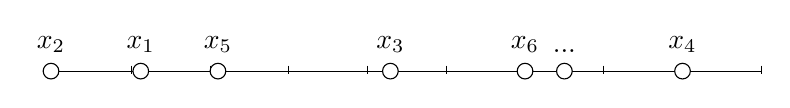
\begin{tikzpicture}
% a straight line segment
\draw (1,0) -- (10,0);
\foreach \x  in {1,...,10}
  \draw[xshift=\x cm] (0pt,2pt) -- (0pt,-1pt);
% the labels
\node[fill=white,draw=black,circle,inner sep=2pt,label=above:{$x_1$}] at (2.12,0) {};
\node[fill=white,draw=black,circle,inner sep=2pt,label=above:{$x_2$}] at (0.98,0) {};
\node[fill=white,draw=black,circle,inner sep=2pt,label=above:{$x_3$}] at (5.29,0) {};
\node[fill=white,draw=black,circle,inner sep=2pt,label=above:{$x_4$}] at (9,0) {};
\node[fill=white,draw=black,circle,inner sep=2pt,label=above:{$x_5$}] at (3.1,0) {};
\node[fill=white,draw=black,circle,inner sep=2pt,label=above:{$x_6$}] at (7,0) {};
\node[fill=white,draw=black,circle,inner sep=2pt,label=above:{...}] at (7.5,0) {};
\end{tikzpicture}
\end{center}

Escogemos el primer elemento $g_1$ de nuestra subsubcesión, y dividimos por la mitad el segmento.

\begin{center}
\begin{tikzpicture}
\draw (1,0) -- (10,0);
\foreach \x  in {1,...,10}
  \draw[xshift=\x cm] (0pt,2pt) -- (0pt,-1pt);
% the labels
\node[fill=black,draw=black,circle,inner sep=2pt,label=above:{$x_1$},label=below:{$g_1$}] at (2.12,0) {};
\node[fill=white,draw=black,circle,inner sep=2pt,label=above:{$x_2$}] at (0.98,0) {};
\node[fill=white,draw=black,circle,inner sep=2pt,label=above:{$x_3$}] at (5.29,0) {};
\node[fill=white,draw=black,circle,inner sep=2pt,label=above:{$x_4$}] at (9,0) {};
\node[fill=white,draw=black,circle,inner sep=2pt,label=above:{$x_5$}] at (3.1,0) {};
\node[fill=white,draw=black,circle,inner sep=2pt,label=above:{$x_6$}] at (7,0) {};
\node[fill=white,draw=black,circle,inner sep=2pt,label=above:{...}] at (7.5,0) {};

\draw[draw=red,ultra thick] (5.5,-1) -- (5.5,1);
\node[text=red] at (5.5,-1.3) {1};
\end{tikzpicture}
\end{center}

En al menos una de las dos mitades del segmento habrá infinitos términos: cogemos esa mitad y repetimos los mismos pasos. Finalmente, llegaremos a una subsucesión de este estilo:

\begin{center}
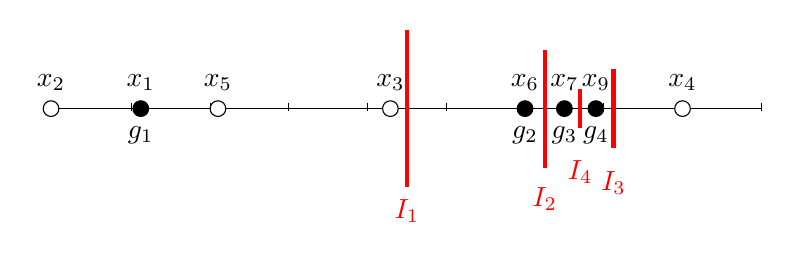
\begin{tikzpicture}
\draw (1,0) -- (10,0);
\foreach \x  in {1,...,10}
  \draw[xshift=\x cm] (0pt,2pt) -- (0pt,-1pt);
% the labels
\node[fill=black,draw=black,circle,inner sep=2pt,label=above:{$x_1$},label=below:{$g_1$}] at (2.12,0) {};
\node[fill=white,draw=black,circle,inner sep=2pt,label=above:{$x_2$}] at (0.98,0) {};
\node[fill=white,draw=black,circle,inner sep=2pt,label=above:{$x_3$}] at (5.29,0) {};
\node[fill=white,draw=black,circle,inner sep=2pt,label=above:{$x_4$}] at (9,0) {};
\node[fill=white,draw=black,circle,inner sep=2pt,label=above:{$x_5$}] at (3.1,0) {};
\node[fill=black,draw=black,circle,inner sep=2pt,label=above:{$x_6$},label=below:{$g_2$}] at (7,0) {};
\node[fill=black,draw=black,circle,inner sep=2pt,label=above:{$x_7$},label=below:{$g_3$}] at (7.5,0) {};
\node[fill=black,draw=black,circle,inner sep=2pt,label=above:{$x_9$},label=below:{$g_4$}] at (7.9,0) {};
\draw[draw=red,ultra thick] (5.5,-1) -- (5.5,1);
\node[text=red] at (5.5,-1.3) {$I_1$};

\draw[draw=red,ultra thick] (7.25,-0.75) -- (7.25,0.75);
\node[text=red] at (7.25,-1.15) {$I_2$};

\draw[draw=red,ultra thick] (8.125,-0.5) -- (8.125,0.5);
\node[text=red] at (8.125,-0.95) {$I_3$};

\draw[draw=red,ultra thick] (7.7,-0.25) -- (7.7,0.25);
\node[text=red] at (7.7,-0.8) {$I_4$};
\end{tikzpicture}
\end{center}

Nuestra subsucesión $\{g_x\}$ es igualmente infinita. Tal y como la hemos definido, tenemos que cada $g_i$ está en un intervalo $(I_i, I_{i-1})$ que cada vez se hace más pequeño. Es decir, que la subsucesión $\{g_x\}$ es de Cauchy y, por lo tanto convergente.

Ahora sólo queda ver cómo podríamos obtener esa subsucesión cuando estamos en espacios que no sean $\real^N$. La idea es sencilla: primero, buscamos una subsucesión que converja en la primera coordenada. Dentro de esa subsucesión, buscamos otra subsucesión que converja además en la segunda, y así con las $N$ coordenadas. 
\end{proof}

\begin{theorem} \label{thmCompactoMax} Sea $K\subset \real$ un conjunto compacto. Entonces, si $\appl{f}{\real}{\real}$ es continua en $K$ existen  $x_m,x_M \in K \tq F(x_m) \leq F(x) \leq F(x_M)\;\forall x \in K$.

Es decir, si $F$ es continua en $K$ alcanza su máximo y su mínimo en el conjunto.
\end{theorem}

\paragraph{Aplicación:}
$F(\gor{x}) = |||\gor{x}|||$ una norma (que ya sabemos que es continua):

\emph{Conclusión:} $m \md{x} \leq |||\gor{x}||| \leq C||\gor{x}||$

\begin{theorem}
En $\real^N$ TODAS las normas son equivalentes. 
\end{theorem}

\subsubsection{Conexión}
\begin{defn}[Conexión\IS por caminos]
Dados $a,b \in C$ podemos encontrar una aplicación continua $\appl{\varphi}{[0,1]}{\real^N}$ tal que $\varphi(0) = a$ y  $\varphi(1) = b$ con $ \varphi(t) \in C\, \forall t \in [0,1]$. 

Es decir, $C$ es conexo por caminos si podemos encontrar una "línea", un camino que una dos puntos cualquiera del conjunto y que además no se salga del conjunto.
\end{defn}

\begin{defn}[Conexión\IS por abiertos]
$C$ es conexo por conjuntos si para cualquier par de abiertos $A,B \subset \real^N \tq C\subset A\cup B$ se cumple que, si $A\cap C\neq \emptyset \y B\cap C \neq \emptyset $ entonces $ A\cap B \neq \emptyset$.

Esto es equivalente a decir que $C$ no puede ser expresado como unión de dos conjuntos disjuntos.
\end{defn}


\begin{remark}

\begin{figure}[hbtp]
\label{imgPeine}
\begin{center}
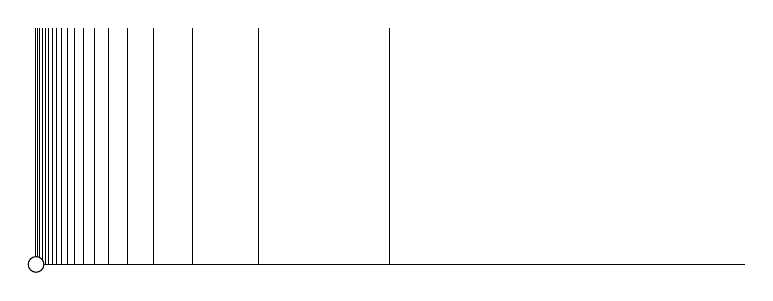
\begin{tikzpicture}

\draw (1,0) -- (10,0);

\foreach \x  in {2,...,20}
  \draw ($10/\x*(1,0) + (0.49,0)$) -- ($(0.49,3) + 10/\x*(1,0)$);

\node[fill=white,draw=black,circle,inner sep=2pt] at (1,0) {};

\end{tikzpicture}
\caption{Conjunto peine}
\end{center}
\end{figure}

Es curioso comprobar que estas 2 definiciones no son equivalentes. Tomemos el conjunto peine (figura \ref{imgPeine})
\[ \left\{(x,0), x\in (0,1]\right\} \cup \{(0,y), y \in (0,1]\} \cup \left\{\bigcup_{n=1}^{\infty}{\left(\frac{1}{n},y\right), y \in [0,1]}\right\} \]

Es un conjunto conexo por abiertos porque no podemos separarlo en dos conjuntos disjuntos. Sin embargo, no es conexo por caminos porque, si queremos ir del punto $(0,1)$ al $(0,0.5)$ no podemos hacerlo ya que el único camino pasaría por el punto $(0,0)$, que no está en el conjunto.
\end{remark}

\subsection{Funciones continuas, abiertos y cerrados}
Sea $F$ continua. Contrario a lo que podríamos intuir, 

1) A abierto $\nimplies F(A)$ abierto.
2) B cerrado $\nimplies F(B)$ cerrado.

\begin{defn}[Función\IS inversa] Dada \[\appl{F}{\real^N}{\real^N}\], definimos su inversa como
\[ \inv{F}(A) = \left\{\gor{x}\in \real^N \tq F(\gor{x})\in A\right\} \]
\end{defn}

\begin{theorem}[Función\IS inversa]\par\noindent\par
\label{thmInversa}
\begin{itemize}
\item F continua $\y$ A abierto $\implies F^{-1} (A)$ abierto.
\item F continua $\y$ B cerrado $\implies F^{-1} (A)$ cerrado.
\end{itemize}
\end{theorem}

Este teorema nos sirve para decir fácilmente si un conjunto es abierto o cerrado. Por ejemplo, consideremos
 \[ M=\{(x,y,z) \in \real^3 \tq x^2 + \cos\left(x\abs{y}\right) - e^z < 1 \} \]

Podemos definir ahí la función $F$ como 
\[ F(x,y,z) = x^2 + \cos\left(x\abs{y}\right) - e^z\]

que va de $\real^3$ a cierto conjunto $A = \{ a \in \real \tq a < 1 \}$. Podemos reescribir $M$ como
\[M=\{(x,y,z) \in \real^3 \tq  F(x,y,z) \in A\}\]

o, de otra forma, $M = \inv{F}(A)$. Según el teorema (\ref{thmInversa}), como $A$ es abierto entonces $M$ también es abierto.

\begin{proof}
1) Dado un $\gor{x} \in F^{-1} (A)$ queremos hallar un $R>0$ tal que $B_R(\gor{x})\subset F^{-1} (A)$. Partimos de 
\[\gor{x}\in F^{-1} (A) \dimplies F(\gor{x})\in A\]

Como $F$ es continua, $\exists \varepsilon>0 \tq B_{\varepsilon}(F(\gor{x}))\subset A$. Esto es equivalente a decir que, para cualquier $\gz$
\[ ||\gor{z}-F(\gor{x})|| < \varepsilon \implies \gor{z}\in A\]

Por la definición de continuidad, dado un $\gor{s}\in B_R(\gor{x})$ 

\[ \exists \delta > 0 \tq ||\gor{x}-\gor{s}||<\delta \implies ||F(\gor{x})-F(\gor{s})||< \varepsilon \]

y por lo tanto $F(\gor{s}) \in A$ y $\gor{s} \in F^{-1} (A)$.
Conclusión: Hemos encontrado un $\delta > 0$ tal que $s \in B_R(\gor{x}) \implies s \in F^{-1} (A)$.

\textit{Pofale. Yo no lo pillo.}
\end{proof}


\subsection{Aplicaciones lineales}

\begin{defn}[Aplicación\IS lineal]

Sea: $\appl{L}{\real^N}{\real^M}$. Entonces, $L$ es lineal si y sólo si

\[ L(\lambda \gor{x}) = \lambda L(\gor{x}) \] 
\[ L(\gor{x}+\gor{y}) = L(\gx)+L(\gy)\] 

\end{defn}
Además, toda aplicación lineal se puede escribir en forma de matriz.

\[L(\gor{x})=A\gor{x} =
\begin{pmatrix}
a_{11} 	& \cdots & a_{1n}		\\
\vdots	& \ddots &  \vdots 	\\
a_{n1}	& \cdots & a_{nn} 
\end{pmatrix}\]

\begin{theorem}
 L lineal $\implies$ L continua.
\end{theorem}
\begin{proof}
 $$L(\gor{x}) = \left(
 \begin{matrix}
  A_1 & \rightarrow \\
  \vdots & \vdots\\
  A_n & \rightarrow
 \end{matrix}\right)$$
 
 COMPLETAR

\end{proof}
\subsection{Norma de matrices}
Consideramos una aplicación

\begin{align*}
\appl{F}{\real^N&}{\real} \\
\gor{x} &\longrightarrow F(\gx) = \underbrace{||A\gx||}_{L(\gx)}
\end{align*}F es continua.

Sabemos que existe $C>0$ tal que $||A\gx|| \leq C||\gx||$, es decir,  $||A\gx||\leq C$ si $||\gx||=1$. Queremos saber cuál es la mejor constante que podemos encontrar, la que más se ajuste. Consideramos el conjunto $M$ de todos los vectores de la esfera unidad, es decir 
$$M = \{||A\gx|| \tq ||\gx||=1\}\subset \real$$
Entonces mejor constante $C$ es la cota superior mínima (supremo) que vamos a llamar $\alpha$. Al ser $F$ continua y $M$ compacto, sabemos que el supremo $\alpha \in M$.

\begin{defn}[Norma\IS de una matriz]
$$\norm{A} = \alpha = \max{\norm{A\gx} \tq \norm{\gx} =1}$$
\end{defn}

\begin{proof} Hay que demostrar que esta norma que hemos definido cumple las propiedades de una norma (\ref{defnNorma}). Las dos primeras son triviales, demostremos la desigualdad triangular
\[ \norm{A+B} = \max{\norm{(A+B)\gx}} = \norm{(A+B)\gx_{A,B}} \] 

donde $\gx_{A,B}$ es el vector que da el valor máximo para esa multiplicación. Usando la propiedad asociativa

\[  \norm{(A+B)\gx_{A,B}} = \norm{A\gx_{AB} + B\gx_{A,B}} ≤ \norm{A\gx_{A,B}} + \norm{B\gx_{A,B}} \]

Sabemos que existen dos vectores $\gx_A$ y $\gx_B$ que maximizan el resultado $\norm{A\gx_A}$ y $\norm{A\gx_B}$ respectivamente, por lo tanto

\[ \norm{A\gx_{A,B}} + \norm{B\gx_{A,B}} ≤ \norm{A\gx_A} + \norm{B\gx_B} = \norm{A} + \norm{B} \]

\end{proof}
%\begin{example}
Calculamos la norma uno de 
\[A = \begin{pmatrix}
      1&2\\-3&1\\2&0
     \end{pmatrix}\]  

Tenemos que maximizar, sabiendo que $|x|+|y| = 1$:

\[ |x+2y| + |-3x+y| + |2x| \leq |x|+|2y| + |3x| + |y| + 2|x| = 6|x|+3|y| \leq 6 (|x|+|y|) =6 \]
¿Podemos encontrar un vector $\gx = (x_0,y_0)$ tal que $||A(x_0,y_0)^T||_1 = 6$?\\
Tomando $x_0 = 1$ y $y_0 = 0$ lo encontramos. Como $\gx$ está en la esfera unidad y es una cota, es el máximo y por lo tanto la norma que buscamos.

Curiosamente, \textbf{coincide con la suma de los valores absolutos de las columnas} y escoger el más grande.
%\end{example}

Si tomamos la norma infinito de 
\[A = \begin{pmatrix}
      1&2\\-3&1\\2&0
     \end{pmatrix}\]

Tenemos que \textbf{coincide con el máximo de las posibles sumas de los valores absolutos de las filas}.

Queremos buscar ahora cuánto vale la norma de una matriz cuando usamos la norma euclídea. Usaremos los dos lemas siguientes para apoyarnos.

\begin{lemma}
 Sea A una matriz cualquiera, entonces $\trans{A}A$ es simétrica.
\end{lemma}
\begin{lemma}
 \[ \underbrace{\pesc{\gx,A\gy}}_{\text{Producto en } \real^n} = \underbrace{\pesc{A^T \gx,\gy}}_{\text{Producto en } \real^M} \]
\end{lemma}

Tenemos $A^TA$ diagonalizable, de dimensión $N \times N$. Buscamos cuánto vale $\norm{A\gx}$ con  $\gx \in \real^N$. Empezamos desarrollando el vector en una base ortonormal de  $A^T A$: \[ \gx = \sum \alpha_i \gv_i \] y por lo tanto \[ ||\gx|| = \sum \alpha_i^2 \pesc{\gv_i,\gv_i}\].
 
 Desarrollamos el producto \[\trans{A}A\gx = \trans{A}A\left(\sum \alpha_i \gv_i\right) = \sum \left(\alpha_i\lambda_i\gor{v}_i\right) \] donde $\lambda_i$ son los autovalres de $\trans{A}A$. 
 
 Ahora queremos hallar el máximo de $||A\gx||$ cuando $||\gx|| = 1$:
 
 \[ ||A\gx||^2 = \pesc{A\gx,A\gx} = \pesc{\trans{A}A\gx,\gx} = \pesc{\sum \lambda_i \alpha_i \gv_i,\sum\alpha_i \gv_i} \]
 
 Como la base de $\{\gv_n\}$ es ortonormal, $\pesc{\gv_i, \gv_j} = 0$ si $i≠j$, por lo tanto sólo nos queda
 \[ \pesc{\sum \lambda_i \alpha_i \gv_i,\sum\alpha_i \gv_i} = \sum \lambda_i \alpha_i^2 \leq \lambda_{max} \left(\sum \alpha_i^2\right) = \lambda_{max} \]
 
 teniendo en cuenta que $\norm{\gx} = 1$ y donde $\lambda_max$ es el autovalor máximo. Es decir, hemos llegado a que
 \[ \max\norm{A\gx} ≤ \sqrt{\lambda_{max}} \]
 
 Hemos definido una cota para $\norm{A\gx}$. Ahora bien, esa cota se alcanza cuando $\gx$ es el autovector asociado a $\lambda_{max}$, por lo tanto la cota es un máximo y la norma de la matriz.
 
 \subsection{Límites}
 
 \begin{defn}[Límite] Dada una función $\appl{F}{\real^N}{\real^M}$, definimos su límite cuando $\gx\to\ga$ de la siguiente forma:
  \[ \lim_{\gx \rightarrow \ga} F(\gx) = \gor{L} \dimplies \forall \varepsilon > 0,  \exists \delta>0 \tlq 0<||\gx-\ga|| <\delta \implies ||F(\gx) - L||<\varepsilon\] 
 \end{defn}
 
 Importante el detalle de $0 < ||\gx-\ga||$, no es un $\leq$, porque no se necesita que la función esté siquiera definida en el punto $\ga$.  
 
 \begin{theorem}[Convergencia\IS de coordenadas]
  
  Sean $\gor{x}_n = (x_1,...,x_n) \in \real^N$ y $\gor{L} = (L_1,...,L_n) \in \real^N$. Entonces
 
  \[ x_n \rightarrow \gor{L} \dimplies (x_1 \rightarrow L_1) \y (x_2 \rightarrow L_2) \y ... \y (x_n \rightarrow L_n) \]
 \end{theorem}
 
 Idea para el cálculo de límites: 
 \begin{itemize}
  \item $\displaystyle\mylim{x}{a}{x} = \lim_{\gy\rightarrow 0} F(\gy+\ga)$.
  \item Límite a lo largo de rectas. $\displaystyle\mylim{x}{a}{\gx} \sim \lim F({t\gor{v}})$
 
 \end{itemize}
 
 Si $\displaystyle\lim F({t\gor{v}})$ toma valores distintos dependiendo de $\gor{v}$ entonces $\nexists \displaystyle\mylim{x}{0}{\gx}$
 
Por otra parte, si $\forall t \in \real, \mylim{x}{a}{t\gor{v}} = L$, entonces $\gor{L}$ es el candidato a ser el límite (no tiene por qué serlo). El siguiente paso sería demostrar con argumentos de comparación (Sandwich) u otros que $\mylim{x}{a}{\gx} = L$.
 
 El contraejemplo para ver que la existencia del límite por rectas no implica la existencia del límite es estudiar la función \[ f(x,y) = \frac{x y^2}{x^2 + y^4}\] . Veamos por qué.
 
 Si os acercamos al límite por medio de rectas:

 \[ f(x,y) = f(x,mx) = \frac{x\cdot(mx)^2}{x^2 + (mx)^4} = \frac{m^2x^3}{(1 + x^2m^4)x^2} \]
 \[ \lim{x\to 0} (f(x,mx)) \rightarrow 0, \forall m \in \real \]

 Pero si nos acercamos al límite por medio de $x = y^2$ tenemos:

\[ f(x,y) = f(y^2,y) = \frac{y^2y^2}{y^4+y^4} = \frac{y^4}{2y^4} = \frac{1}{2} ≠ 0\]  

Por lo tanto, el límite no existe a pesar de que existe cuando nos acercamos por rectas.
 
 
\begin{theorem}
 $F$ es continua si y sólo si para cualquier abierto $A$, $F^{-1}(A)$ es abierto.
\end{theorem}
\obs
Si $\appl{F}{\omega\subset\real^N}{\real^M} \dimplies$ para cualquier abierto $A, F^{-1}(A) = \omega \cup V$, con $V$ abierto.

\begin{proof}
De este teorema ya teníamos demostrada la implicación a la derecha (\ref{thmInversa}), así que sólo falta demostrar hacia la izquierda. Queremos probar que

\[ \forall \varepsilon > 0\; \exists \delta>0 \tlq ||\gx-\ga||<\delta \implies ||F(\gx)-F(\ga)||<\epsilon \]

Tomamos  \[ A = B_{\varepsilon}(F(\ga))\] de tal forma que \[ F(\ga) \in A \implies \ga \in F^{-1}(A) \]

Por hipótesis, $F^{-1}(A)$ abierto y $\ga \in F^{-1}(A)$ . Entonces 
\[\exists B_{\delta}(\ga) \subset F^{-1}(A) \].Es decir, \[ \gor{s}\in B_{\delta}(\ga) \subset F^{-1}(A), s\in F^{-1}(A) \implies F(s) \in A = B_{\varepsilon}(F(\ga))\]
\end{proof}

\begin{remark}
Este teorema también se cumple para cerrados.
\end{remark}


\section{Diferenciación}

\begin{defn}[Función\IS diferenciable]
 $F$ diferenciable en $\gor{a}$ si 
 
 $$\exists \text{ aplicación lineal L} \tlq \frac{F(\gx)-F(\ga)-L(\gx-\ga)}{||\gx-\ga||} \underbrace{\rightarrow}_{\gx\rightarrow\ga} 0$$
$$ = \lim_{\gor{h} \rightarrow \gor{0}} \frac{\md{F(\ga+\gor{h}) - F(\ga) - L\gor{h}}}{||\gor{h}||}$$

\end{defn}


\obs
\begin{itemize}
\item Si existe, $L$ es única.
\end{itemize}

\begin{proof}
Supongamos que existen $L_1,L_2$.
\[0=\lim_{\gor{h} \rightarrow \gor{0}} \frac{F(\gor{a}+\gor{h}) - F(\ga)-L_1\gor{h}}{||\gor{h}||} = \lim_{\gor{h} \rightarrow \gor{0}} \frac{F(\gor{a}+\gor{h}) - F(\ga)-L_2\gor{h}}{||\gor{h}||}\].

$$\text{ Sumando: } 0 = \lim_{\gor{h} \rightarrow \gor{0}} \frac{||F(\gor{a}+\gor{h}) - F(\ga)-L_1\gor{h}|| + ||F(\gor{a}+\gor{h}) - F(\ga) -L_2\gor{h}||}{||\gor{h}||}$$

\obs $||A-B|| = ||A+(-B)|| \leq ||A||+||B||$

$$\leq \lim_{\gor{h} \rightarrow \gor{0}} \frac{2\cdot\md{F(\ga + \gor{h}) - F(\ga)} + \md{L_1\gor{h}} + \md{L_2\gor{h}}}{\md{\gor{h}}}$$

Completar la contradicción.
\end{proof}

\paragraph{Notación: (Diferencia de $F$ en $\ga$)}

$$L\equiv DF(\ga)$$ 

\paragraph{Proposición:}
$$F \text{ diferenciable en } \ga \implies F \text{ continua en } \ga$$
\begin{proof}
 $$\lim_{\gor{h} \rightarrow \gor{0}} \frac{\md{F(\ga+\gor{h}) - F(\ga) - L\gor{h}}}{\md{\gor{h}}} = 0$$
 Esta es la definición de diferenciable. Para que este límite sea 0, el numerador tiene que tender a 0, por lo que $F(\ga+\gor{h}) - F(\ga) \rightarrow 0$
\end{proof}

\obs
$F$ diferenciable en $\ga$.

$\appl{F}{\real^N}{\real^M}$

Sabemos:
 $$0 = \lim_{\gor{h} \rightarrow \gor{0}} \frac{||F(\ga+\gor{h}) - F(\ga) - L\gor{h}}{||\gor{h}||} = 0 $$
 
 En particular (tomando  h = $t \gor{e_1})$

$$ \lim_{\gor{t} \rightarrow \gor{0}}\frac{a}{b} = \lim_{\gor{t} \rightarrow \gor{0}}\norm{\underbrace{\frac{1}{t} F(\ga+t\gor{e_1})-F(\ga))-L\gor{e_1}}_{\gor{W}(t)\in\real^N}}$$
 Tomando la componente k-esima:
\begin{gather*}
 0 = \mylim{t}{0}{\frac{F_K(a+te_i)-F_k(a)}{t} - L_{ki}}\\
 L_{ki} = \mylim{t}{0} {\frac{F_k(a+te_i) - F_k(a)}{t}} = \deriv{ F_k}{x_i}(\ga)
\end{gather*}

\paragraph{Nomenclatura: }
Aproximación lineal $\sim$ Diferencial.

Matriz jacobiana $\sim$ Jacobiana.

\begin{theorem}
 Matriz asociada a $DF(\ga) \equiv $ Matriz de las derivadas parciales de F.
 
 $$DF(\ga) \equiv \begin{pmatrix}
                \dpa{F_1}{x_1} & \cdot & \dpa{F_1}{x_N}\\
                \vdots& \ddots & \vdots\\
                \dpa{F_N}{x_1} & \cdot & \dpa{F_N}{x_N}
                \end{pmatrix}
$$
\end{theorem}

\begin{theorem}
 $F$ diferencialbe en $\ga \implies \exists \deriv{F_k}{x_i}(\ga), i=1,2,...,N \y k = 1,2,...,M$
\end{theorem}

El contraejemplo para demostrar $\Leftarrow$ es el mismo que en los límites a lo largo de rectas.

$f(x,y) = \left\{ \begin{matrix}

\frac{xy^2}{x+y^2} & (x,y) = (0,0) \\ 
0 & (x,y)=(0,0)
           
          \end{matrix}\right.
$
\paragraph{Comentarios sobre notación: }
\begin{itemize}
 \item $\appl{\delta}{\real}{\real^M}$. Utilizamos notación vectorial en vez de matricial (porque tendríamos una matriz columna).\\
 Ejemplo: la velocidad (en un instante de tiempo, un punto en el espacio).
 \item $\appl{F}{\real^N}{\real}$ (función escalar):

 COMPLETAR
 Se suele llamar vector gradiente.
 \item 
\end{itemize}

\subsection{Regla de la cadena: }
\paragraph{Derivada de una composición:\\}

COMPLETAR DIBUJITO

$\appl{F}{\real^N}{\real^M}$. 

$\appl{G}{\real^M}{\real^K}$.

$\appl{H=G\circ F}{\real^N}{\real^K}$.

$ \gx \in \real^N, \gy \in \real^M$

$F$ diferenciable en $\ga$, $G$ diferenciable en $F(\gor{a})$. Entonces $H=G\circ F$ es diferenciable en $\ga $.
Además la expresión matricial es:

$\underbrace{DH(\ga)}_{K\times N} = \underbrace{DG(F(\ga))}_{K\times M}\cdot \underbrace{DF(\ga)}_{M\times N}$
 
\obs
\paragraph{Notación de Leibniz:}

Para calcular 1 único elemento de la matriz diferencial (el de la fila $i$, columna $j$):

$$\deriv{H_i}{x_j}(\ga) = \displaystyle\sum_{k=1}^M \deriv{G_i}{y_k}\cdot\deriv{F_k}{x_j}$$
Con cuidado de $\displaystyle \deriv{G_i}{y_k}$ evaluado en $\displaystyle F(\ga)$ y $\displaystyle\deriv{F_k}{x_j}$ evaluado en $\ga$.

\paragraph{Aplicaciones y ejemplos:}
\begin{itemize}
 \item 
 $\appl{F}{\real^N}{\real}$
 
 $\appl{\sigma}{\real}{\real^N}$
 
 Sea $g\equiv F\circ \sigma \equiv \text{ Comportamiento de F a lo largo de la curva } \sigma, \appl{g}{\real}{\real}$.

$$g'(t_0) = DF(\sigma(t_0))D\sigma(t_0) = \underbrace{...}_{\text{Notación matricial}} = \underbrace{\pesc{\nabla F(\sigma(t_0))}{\sigma'(t_0)}}_{\text{Notación vectorial}}$$

 
 \item 
 $\sigma(t) = t\gor{b} + (1-t)\ga$
 
 $\appl{F}{\real^N}{\real^M}$
 
 $F\circ \sigma(t) \equiv g(t)$
 
 COMPLETAR
\end{itemize}

\subsection{Extensiones del teorema del Valor Medio}
\begin{itemize}
 \item Original:
 $\appl{f}{\real}{\real}$ diferenciable. 
 
 $f(b)-f(a) = f'(c)(b-a)$ para algún $c\in[a,b]$
 
 \item
  
 $F : \real^N  \longrightarrow \real$
 
 $\sigma(t)  = t(\gor{b})+(1-t)\gor{a}$
 
 $g  = F\circ \sigma$
 $\appl{g}{\real }{\real}$
 
 $F(\gor{b}-\gor{a}) = g(1)-g(0)  = g'(s) \text{ para algún }s\in[0,1]$
 
  
  Peeeeero...
  $$\appl{F}{\real^N}{\real^2}$$
  $$F(\gor{b})-F(\ga) = \begin{pmatrix}
                         \pesc{\nabla F_1(\gor{c_1}),{\gor{b}-\ga}}\\
                         \pesc{\nabla F_2(\gor{c_2}),\gor{b}-\ga}
                        \end{pmatrix}
$$
  Tenemos 2 $c$ distintos, uno para cada $f$, por lo que este teorema pierde sentido.
  
  \item Versión para funciones matriciales:
  
  \begin{theorem} [Extensión del valor medio]
  Sea $f \in C^1$ en un abierto que contenga $[a,b]$.
  $$\norm{F(\gor{b}-\ga)} \leq |||DF(\gor{c})|||\cdot\norm{\gor{b}-\ga}$$ 
  
  Siendo c un punto del segmento que une $\ga$ y $\gb$ en el que $|||DF(tb+(1-t)a)|||$ alcanza su máximo.
   
  \end{theorem}

  
  
  \begin{proof}
   i) $$\appl{f}{\real}{\real}$$
   $$f(\gor{b}-f(\ga) = g(1)-g(0) = \int_0^1g'(s)ds \text{ con } g(t) = f(tb+(1-t)a)$$
   
   ii)  $$\appl{h}{\real^N}{\real}$$
   $$h(\gor{b}-h(\ga) = g(1)-g(0) = \int_0^1g'(s)ds = \int_0^1 \pesc{\nabla h(s\ga+(1-s)\gor{b}),(\gor{b}-\ga)}$$
   $$g(t) = h(tb+(1-t)a)$$
   
   iii) $$\gor{G} = (G_1,...,G_M), G_i = \int_0^1H_i(t)dt$$
   Con $\gor{H} = (H_1(t),...,H_M(t))$
   
   
   $$\norm{\gor{G}}^2 = \pesc{\gor{G},\gor{G}} = \sum_{i=1}^M \left(\int_0^1 H_i(t)dt\right) \underbrace{\left(\int_0^1 H_i(s)ds\right)}_{G_i}$$
 
   $$\norm{\gor{G}}^2 = \displaystyle\int_0^1 \left(\underbrace{\sum_{i=1}^M G_i H_i (t)}_{\pesc{\gor{G},\gor{H}(t)}\leq \norm{\gor{G}}\cdot \norm{\gor{H}}}\right)dt$$
   Conclusión:
   $$\norm{\gor{G}}^2 \leq \displaystyle\int_0^1\norm{G}\cdot\norm{H(t)}dt$$
   
   iv) $\appl{F}{\real^N}{\real^M}$
   
   $\appl{F_i}{\real^N}{\real}$
   
   $\underbrace{F_i(\gor{b})-F_i(\ga)}_{G_i} = \displaystyle\int_0^1 \underbrace{\pesc{\nabla F_i (s\gor{b}+(1-s)\ga ),(\gor{b}-\ga)}}_{H_i(t)}dt$
   
   Por el apartado iii tenemos que:
   
   
   $$\gor{H}(t) = \begin{pmatrix}
                   H_1(t)\\
                   \vdots\\
                   H_M(t)
                  \end{pmatrix}
                = \begin{pmatrix}
                   \pesc{\nabla F_1(tb+(1-t)a),b-a}\\
                   \vdots\\
                   \pesc{\nabla F_M(tb+(1-t)a),b-a}
                  \end{pmatrix}
		= \left(DF(...)\right)\begin{pmatrix}
		                        b_1-a_1\\
		                        \vdots\\
		                        b_M-a_M
		                       \end{pmatrix}
$$

$$\norm{H(t)} = \norm{DF(...)(\gor{b}-\ga)} \leq \norm{DF}\cdot\norm{\gor{b}-\ga}$$


$$\norm{F(\gor{b})-F(\ga)} \leq \displaystyle\int_0^1 \norm{\nabla DF_i(tb+(1-t)a),b-a}dt$$

Aplicando: $A\gor{v} \leq |||A|||\cdot \norm{\gor{v}}$

$$\norm{F(\gor{b})-F(\ga)} \leq \displaystyle\int_0^1 |||DF(*)|||\cdot\norm{\gb-\ga}dt$$
$$= \norm{\gb - \ga} \displaystyle \int_0^1 |||DF(tb+(1-t)a)||| dt \leq |||DF(\gor{c})|||\cdot\norm{\gb-\ga}$$ 

Siendo c un punto del segmento que une $\ga$ y $\gb$ en el que $|||DF(tb+(1-t)a)|||$ alcanza su máximo.
   
Conclusión:

$$\norm{F(\gor{b})-F(\ga)} \leq \norm{DF}\cdot\norm{\gor{b}-\ga}$$
  \end{proof}

\end{itemize}

\paragraph{Aplicación:\\}

$\appl{F}{\real^N}{\real^M}, F \in C^1$, definida en un conjunto abierto y conexo.

$DF(\gx) \equiv 0, \forall \implies F \equiv $ cte.	

\subsection{Derivada direccional: }

$\appl{F}{\real^N}{\real^M}$ (escalar)

$\ga \sim$ Recta que pasa por $\ga$ con dirección $\gor{v}$.

$r(t) = \ga + t\gor{v}$. 

\obs
Como una recta tiene infinitos vectores directores (dependiendo de la longitud), siempre tomaremos vectores directores unitarios, con $\norm{\gor{v}} = 1$.


Vamos a estudiar: $g(t) = F(\ga + t\gor{v}) = F \circ r (t)$.

$t \sim 0 \dimplies \ga + t\gor{v} \sim \ga$
\begin{defn} [Regla de la cadena]
$$g'(0) = \displaystyle\lim_{h \rightarrow 0} \frac{g(h)-g(0)}{h} = \displaystyle\lim_{h \rightarrow 0} \frac{F(\ga+h\gor{v})-F(\ga)}{h} \equiv D_{\gor{v}}F(\ga)$$. 
\end{defn}

\obs
La existencia de $D_{\gor{v}}F(\ga), \forall \gor{v}\in \real^N$ NO garantiza que $F$ sea derivable.


Si sabemos que $F$ SÍ es diferenciable podemos usar la regla de la cadena obteniendo:

$D_{\gor{v}}F(\ga) = g'(0) = D(F\circ r)(0) = ... = \pesc{\nabla F(\ga),\gor{v}}$


\paragraph{Aplicación:} 
\begin{itemize}
 \item 
 Dirección de máximo crecimiento:

$D_{\gor{v}}F(\ga) = \pesc{\nabla F(\ga),\gor{v}}\leq \norm{\nabla F(\ga)}\cdot \underbrace{\norm{\gor{v}}}_{\equiv 1}$

Conclusión:
\begin{align*}
D_{\gor{v}}F(\ga) &\leq \norm{\nabla F(\ga)}\\
&\uparrow\\
\text{El }= \text{se obtien}&\text{e cuando }\gor{v} = \displaystyle \frac{\nabla F(\ga)}{\norm{\nabla F(\ga)}}. 
\end{align*}

 
 \item
 Vector perpendicular a los conjuntos de nivel
 
 $\appl{F}{\real^N}{\real^M}$
 
 $S = \{ \gx \in \real^N \tq F(\gx) = 0\}$ (Conjunto de nivel)
 
 $\ga \in S$
 
 Entonces: $\nabla F(\ga) \perp S$
\end{itemize}

\begin{theorem}[Derivadas parciales continuas implican función diferenciable]
Si existen todas las derivadas parciales y son continuas $\implies F$ diferenciable en $\ga$.
 
\end{theorem}

Contraejemplo de la no reciprocidad: $f(x) = x^2 sin\left(\frac{1}{x}\right)$

\begin{proof}
 $\appl{F}{\real^2}{\real}$
 
 $$¿\frac{\left|F(a+a,b+k) - F(a,b) - \deriv{F}{x}(a,b) h - \deriv{F}{y}(a,b)k\right|}{\norm{(h,k)}}\longrightarrow 0?$$
 
 Sumamos y restamos al numerador $F(a,b+k)$.
 
 $$\frac{\left|\left(\underbrace{F(a+h,b+k) - F(a,b+k)}_{\deriv{F}{x}(a+\tilde{h},b+k) \text{ para algún } 0 \leq\tilde{h}\leq h} -  \deriv{F}{x}(a,b) h\right) + \left(\underbrace{F(a,b+k) - F(a,b)}_{\deriv{F}{x}(a+h,b+\tilde{k}) \text{ si } 0 \leq\tilde{k}\leq k}- \deriv{F}{y}(a,b) k\right)\right|}{\sqrt{h^2+k^2}}$$

 $$0\leq\frac{\left|\deriv{F}{x}(a+\tilde{h},b+k)-\deriv{F}{x}(a,b)\right| \cdot |h| + \left| \deriv{F}{y}(a,b+\tilde{k}) - \deriv{F}{y}(a,b)\right| \cdot |k|}{\sqrt{h^2+k^2}} = (*)$$
 
 Aquí es donde aplicamos que las derivadas parciales son continuas: como $h$ y $k$ son pequeños (por lo tanto $\tilde{h}<h$ también lo será) los puntos $(a,b)$ y $(a+h,b+k)$ también están cerca, por lo que sus imágenes por la derivada estarán también cerca, es decir, $|\deriv{F}{x}(a,b)-\deriv{F}{x}(a+\tilde{h},b+k)| \rightarrow 0$ y lo mismo con la otra.
 
 Conclusión:
 
 \begin{align*}
0 \leq (*) \leq \varepsilon \frac{|h|+|k|}{\sqrt{h^2+k^2}} &\leq C\varepsilon \rightarrow 0 \text{ cuando } \gor{h},\gor{k} \rightarrow \gor{0}\\
&\uparrow\\
\text{El numerdador es la} & \text{ norma 1 y el denominador la norma 2.}\\
\text{En } \real^N &\text{ todas las normas son equivalentes.}  
 \end{align*}
 
 
\end{proof}


\subsection{Derivadas iteradas:}

\paragraph{Notación:}

$\deriv{}{y}\left(\deriv{f}{x}\right) \equiv \deriv{^2f}{x \partial y}$

\begin{theorem}[Euler (orden de las derivadas)]
Si las derivadas segundas son continuas, entonces:
$$\deriv{^2f}{x_i\partial x_j} = \deriv{^2 f}{x_j \partial x_i}$$
\end{theorem}

\subsection{Máximos y mínimos}

\index{Máximo/mínimo!local}
\begin{defn}[Máximo/mínimo local] Sea $\appl{f}{\real^N}{\real}$. Diremos que $\vx_0 \in \real^N$ es un punto de máximo local si $\exists \epsilon > 0 \tq F(\vx_0) \geq F(\vx)\;\; \forall \vx \in B_{\epsilon} (\vx_0) $

La definición es análoga para el mínimo\end{defn}

\begin{remark} Por las propiedades del gradiente, si $F$ es diferenciable y $\vx_0$ es un máximo o mínimo local, entonces debe ser $\nabla F(\vx_0) = \vec{0}$.\end{remark}

\index{Punto!crítico}
\begin{defn}[Punto crítico] $\vx \in \real^N$ es un punto crítico de $F$ si y sólo si $\nabla F(\vy) = \vec{0}$\end{defn}

No todos los puntos críticos son máximos o mínimos, así que tenemos que clasificarlos de alguna forma. Para ello, usamos el polinomio de Taylor de orden 2, de forma que 

\[F(x,y) = F(x_0, y_0) + \pesc{\nabla F(x_0, y_0), (x-x_0, y-y_0)} +\]\[\frac{1}{2}(x-x_0, y-y_0)\left(\begin{matrix} \frac{\partial^2 f}{∂ x^2} (x_0,y_0) & \frac{\partial^2 f}{\partial x \partial y} (x_0,y_0) 
\\ \frac{\partial^2 f}{\partial y \partial x} (x_0,y_0) & \frac{\partial^2 f}{\partial y^2} (x_0,y_0) \end{matrix}\right) \left(\begin{matrix} x - x_0 \\ y - y_0 \end{matrix}\right) + \epsilon \]

Simplificando nos queda que:

\[F(\vx) = F(\vx_0) + \pesc{\nabla F(\vx_0),\vx - \vx_0} + \frac{1}{2}(\vx - \vx_0) D^2F(\vx_0) (\vx - \vx_o) ^T + \epsilon\]

Dado que el gradiente es 0, el punto clave es el signo de $\frac{1}{2}(\vx - \vx_0) D^2F(\vx_0) (\vx - \vx_o) ^T$. Para ello, usamos las siguientes definiciones del álgebra lineal.

\subsubsection{Resultados de álgebra lineal}
\index{Matriz!semidefinida positiva/negativa}
\index{Matriz!definida positiva/negativa}
\begin{defn}[Matriz semidefinida y definida positiva y negativa]\noindent\\ \indent
La matriz $A$ de dimensión $N\x N$ es semidefinida positiva si y sólo si $\vv A \vv^T \geq 0 \;\; \forall \vv \in \real^N$.

La matriz $A$ de dimensión $N\x N$ es definida positiva si y sólo si $\vv A \vv^T > 0 \;\; \forall \vv ≠0 \in \real^N$.

La matriz $A$ de dimensión $N\x N$ es semidefinida negativa si y sólo si $\vv A \vv^T \leq 0 \;\; \forall \vv \in \real^N$.

La matriz $A$ de dimensión $N\x N$ es definida negativa si y sólo si $\vv A \vv^T < 0 \;\; \forall \vv ≠0 \in \real^N$.
\end{defn}

\begin{theorem}
Si una matriz es simétrica, existe una base en la cual la matriz es diagonal.
\end{theorem}

\index{Autovalor}
\index{Autovector}
Sea $A$ una matriz $N\x N$. Entonces diremos que un vector $\vv ≠ \vec{0}$ es un autovector asociado al autovalor $\lambda\in \real$ si y sólo si $A\vv = \lambda\vv$. Dado que podemos escribir

\[ A = \left(\begin{matrix}
a & b \\ c &  d
\end{matrix}\right)\;\;\;\; \vv = \left(\begin{matrix}
x\\ y
\end{matrix}\right) \], entonces tenemos que $A\vv = \lambda \vv$ si y sólo si

\[ \left\lbrace\begin{matrix}ax+by=\lambda x \\ cx+dy = \lambda y \end{matrix}\right. \]

Es decir, la autorrecta $\begin{pmatrix} x \\ y \end{pmatrix}$ es una solución no trivial del sistema anterior. Sin embargo, para que haya soluciones no triviales el determinante de la matriz $\begin{pmatrix}a-\lambda & b \\ c & d - \lambda\end{pmatrix}$ debe ser 0.

Por lo tanto, los autovalores son las soluciones de la ecuación $det(A-\lambda I) = 0$, siendo $I$ la matriz identidad.

\begin{theorem}
Si un conjunto de autovectores es una base, entonces la matriz $A$ expresada respecto a esa base pasa a ser diagonal, y los elementos de la diagonal son los autovalores. 

Si dos autovalores son distintos, los autovectores asociados son distintos.

Si A es simétrica, entonces el conjunto de autovectores es una base.
\end{theorem}

Volvemos ahora al cálculo.

\begin{theorem}[Clasificación de puntos críticos]
Sea $\appl{F}{\real^N}{\real}$, $F\in C^2$ (con dos derivadas continuas), y sea $\vx_0$ un punto crítico. Entonces

\begin{enumerate}
\index{Máximo/mínimo!local}
\index{Punto!de silla}
\index{Punto!crítico degenerado}

\item Si \textbf{todos} los autovalores de $D^2F(\vx_0)$ son \textbf{mayores que cero}, entonces $D^2F(\vx_0)$ es definida positiva y $\vx_0$ es un \textbf{mínimo local}.
\item Si \textbf{todos} los autovalores de $D^2F(\vx_0)$ son \textbf{menores que cero}, entonces $D^2F(\vx_0)$ es definida negativa y $\vx_0$ es un \textbf{máximo local}.
\item Si \textbf{algunos} autovalores son \textbf{mayores que cero} y otros son \textbf{menores que cero}, entonces $\vx_0$ es un \textbf{punto de silla.}
\item Si algún autovalor \textbf{es 0}, y el resto son mayores o menores que cero, entonces $\vx_0$ es un \textbf{punto crítico degenerado}.
\end{enumerate}
\end{theorem}

\subsubsection{Ejemplos}

Tomamos $F(x,y) = x^2 + y^2 +xy$. Obtenemos los puntos críticos, es decir, los puntos en los que $\nabla F(x,y) = (0,0)$. El punto resultante es $(0,0)$. Estudiamos el tipo de punto crítico. Para ello, calculamos la matriz hessiana en ese punto:

\[ D^2F(0,0) = \begin{pmatrix}2&1\\1&2\end{pmatrix}\]. 

Los autovalores son las soluciones de

\[ 0 = det\left(\begin{pmatrix}2&1\\1&2\end{pmatrix} - \lambda \begin{pmatrix}1&0\\0&1\end{pmatrix}\right) = det\begin{pmatrix}2-\lambda & 1 \\ 1 & 2-\lambda\end{pmatrix} = (2-\lambda)^2  - 1\]

Por lo tanto, $\lambda$ es $3$ o $1$. Dado que ambos autovalores son mayores que 0, entonces $D^2F$ es definida positiva y $(0,0)$ es un mínimo local.

\subsection{Máximos y mínimos absolutos}

\index{Máximo/mínimo!absoluto}
\begin{defn}[Máximo y mínimo absoluto] Sea $\appl{F}{\real^N}{\real}$ y $A\subset \real^N$. $\vx_m$ es un máximo absoluto de $F$ en $A$ si y sólo si $F(\vx_m) ≥ F(\vx)\;\; \forall \vx \in A$. La definición es análoga para el mínimo.
\end{defn}

\begin{theorem}[Teorema de compacidad]
Tenemos un conjunto $K\subset \real^N$ compacto (cerrado y acotado). Supongamos la sucesión $\{\vx_n\}_{n\in\nat}\subset K$. Entonces podemos encontrar al menos una subsucesión $\{\vx_{n_j}\}_{j\in\nat} \subset \{\vx_n\}_{n\in\nat}$ tal que $\{\vx_{n_j}\}$ es convergente.
\end{theorem}

\begin{proof}
Trabajamos en dimensión 2, pero la demostración es análoga.
Como $K$ es compacto, podemos encontrar un cuadrado $Q_0$ de lado $L$ que encierre completamente a $K$. Divido $Q_0$ en $2^2$ cuadrados de lado $L/2$.  En alguno de ellos hay infinitos términos de la sucesión: lo llamamos $Q_1$ y me quedo con uno de los términos de la sucesión, al que llamamos $x_1$. Volvemos a dividir este cuadrado en cuatro cuadrados, elegimos uno que tenga infinitos términos de la sucesión y seleccionamos un elemento de la sucesión dentro al que llamamos $x_2$. Repetimos esto muchas veces, de forma que cada término $x_n$ está encerrado en el cuadrado $Q_n$ de lado $\frac{L}{2^n}$. 

Si $k,l > n$, entonces es claro que $\md{\vx_k-\vx_l}$ es menor o igual que la diagonal de $Q_n$, que es $\frac{L}{2^n}\sqrt{2}$, que tiende a cero cuando $n\to\infty$. Por el criterio de Cauchy, entonces esta sucesión es convergente, y como $K$ es cerrado el límite pertence a $K$.
\end{proof}

\begin{theorem}
Sea $K\subset \real^N$ compacto y $\appl{F}{\real^N}{\real}$, continua en $K$. Entonces, $F$ alcanza su máximo y mínimo absolutos en $K$.
\end{theorem}

\begin{proof}

Como $F$ es acotada, existe $\alpha = \sup \{ F(x) \tq x \in K\}$. Existe entonces una sucesión $\{x_n\}$ tal que si $n\to \infty$ entonces $F(x_n)\to \alpha$. 
Sabemos que existe $\{x_n\}\subset K$, por lo que existe una subsucesión$\{x_{n_j}\}$ convergente tal que $x_{n_j} \to x_0 \in K$

Como $F$ es continua, $F(x_{n_k})\to F(x_0)$, es decir $F(x_{n_j}) \to \alpha$, por lo tanto el supremo es el máximo.
\end{proof}

\subsubsection{Ejemplos}

La función a estudiar es $F(x,y) = x^2-y^2$ en la bola $\omega = \{ x^2 + y ^2 ≥ 1\}$. Es diferenciable en todo $\real$ porque es un poliniomio. 

Calculamos el diferencial y vemos qué ocurre cuando es 0 \[\nabla F = (2x, -2y) = (0,0) \implies (x,y) = (0,0)\]

Operando, vemos que el punto $(0,0)$ es un punto de silla. Ahora sólo queda ver el comportamiento en la frontera $C$, cuando $x^2+y^2 = 1$. $F$ restringida a $C$ quedaría de la siguiente forma:

\[ F(\cos t, \sin t) = \cos^2 t - \sin^2 t = \cos 2t\]

El coseno tiene máximos cuando $t=0$ y $t=\pi$, y mínimos cuando $t=\pi /2$ y $t=3\pi /2$. Es decir, tiene máximos absolutos en los puntos $(1,0),\;(-1,0)$ y mínimos absolutos en $(0, -1)$, $(0, 1)$. 

\index{Multiplicadores de Lagrange}
\begin{theorem}[Multiplicadores de Lagrange]
Tenemos una función $\appl{F}{\real^2}{\real}$ y una restricción $G(x_1,\cdots,x_n) = k$, resolvemos el siguiente sistema:

\begin{align*}
\nabla F &= \lambda \nabla G \\
G &= k
\end{align*} 

\end{theorem}


\subsection{Desarrollo de Taylor}

$\appl{F}{\real^N}{\real}. F\in C^k$\footnote{F es k veces derivable}. 

Queremos desarrolar $F$ alrededor de $\ga \in \real^N$.

Dimensión 1) $g(x) = g(0) + g'(0)x + \frac{g''(0)}{2!}x^2 + ... + \frac{g^{k)}(0)}{k!}x^k + \underbrace{error}_{\frac{g^{k+1)}(s)}{(k+1)!}x^{(k+1)}}$

$F(\ga + \gor{h}) = F(\ga) + ...$

Más dimensiones) 

Tomamos $g(t) \equiv F(t(\ga + \gor{h}) + (1-t)\ga)$. Así hemos reducido el cálculo a dimensión 1.

%\begin{gather}

$$g'(t) = \pesc{\nabla F(a+th),h} = \sum_{i=1}^N \deriv{F}{x_i}(a+th)\cdot h_i$$
$$g'(0) = \pesc{\nabla F(\ga), \gor{h}}$$
$$g''(t) = \sum_{i=1}^N\left(\sum_{j=1}^N \deriv{}{x_j}\deriv{F}{x_i}(\ga+\gor{h})\cdot{h_j}\right)h_i = \sum_{i,j = 1}^N \deriv{^2F}{x_i \partial x_j}(\ga+t\gor{h})h_ih_j $$

Iterando:

$$\frac{g^{s)} (0)}{s!} = \frac{1}{s!}\sum_{i_1,i_2,...,i_s=1}^N \frac{\partial^s F}{\partial x_{i_1},x_{i_2},...,x_{i_s}}
$$%\end{gather}
                                                                                          
El hesiano aparece en:
$$g''(t) = \sum_{i=1}^N\left(\sum_{j=1}^N \deriv{}{x_j}\deriv{F}{x_i}(\ga+\gor{h})\cdot{h_j}\right)h_i = \sum_{i,j = 1}^N \deriv{^2F}{x_i \partial x_j}(\ga+t\gor{h})h_ih_j = ... =
$$$$\frac{1}{2} (h_1,...,h_N) \cdot \left(D^2F(\ga)\right) \cdot \begin{pmatrix}
h_1\\
\vdots\\
h_N                                                                                                                                                                                                                                       \end{pmatrix}
$$

\paragraph{Desarollo de Taylor en general:}

$$F(\gor{a}+\gor{h}) = F(\ga) + \pesc{\nabla F(\ga),\gor{h}} + \frac{1}{2} \gor{h}^T D^2F(\ga)\gor{h} + \frac{1}{3!}\sum_{i,j,k=1}^N \frac{\partial^3F}{\partial x_k,\partial x_j, \partial x_i} (\ga) h_kh_jh_i + $$

\begin{theorem}
 $$\frac{|F(\ga+\gor{h} - P_{s,a}(\gor{h})|}{\norm{\gor{h}}^s} \rightarrow 0, \text{ Cuando } \gor{h} \rightarrow 0$$
 Además $P_{s,a}(\gor{h}$ es el único polinomio de orden S que hace que el límite sea 0).
\end{theorem}

Con estos conocimientos son posibles de realizar todos los ejercicios de la hoja de problemas 2.


\section{Teoremas de la función implícita y la función inversa}

En el mundo lineal tenemos: 

\begin{itemize} \item $\appl{F}{\real^N}{\real^N}$ y 
$L(\gx) = A\gx,  A = $ matriz $NxN$


Si queremos resolver el sistema: $A\gx = \gy$ sabiendo que $A\gor{0} = \gor{0}$.\\ Este sistema tiene solución $\dimplies \det(A) \neq 0$ (porque $\exists A^{-1}$).
\item
$\appl{F}{\real^{N+M}}{\real^N}$

$L(\gx) = A\gx, A = $ matriz $Nx(N+M)$

Para resolver el sistema $A\gx = \gy$.  Se resolvía parametrizando $M$ variables.

\item En el mundo NO lineal:
$\appl{F}{\real^N}{\real^N}$

Suponemos que $\exists F(\ga) = F(\gor{b})$

$\left.\begin{matrix}
F(x_1,\dotsc,x_N) = y_1\\
F(x_1,\dotsc,x_N) = y_2\\
\vdots\\
F(x_1,\cdots,x_N) = y_N          
        \end{matrix}
\right\} F(\gx)=\gy$
\end{itemize}

Vamos a intentar resolver este problema utilizando Taylor para aproximar al orden lineal, pero tenemos que pagar un precio: para que taylor funcione tenemos que trabajar cerca del punto. Esto significa que el resultado va a ser local.


\begin{theorem}[Teorema\IS de la aplicación contractiva]
Sea $\appl{F}{\real^N}{\real^N}$ o\\
Sea $\appl{F}{C}{C}, C\in \real^N$, cerrado, o\\
Sea $\appl{F}{K}{K}, K\in \real^N$, compacto.

Supongamos que existe $\alpha\in(0,1) \tlq$

$$\md{F(x)-F(y)}\leq \alpha\md{x-y} \forall x,y \in \left\{\begin{matrix}
                                                           \real^N\\
                                                           C\\
                                                           K
                                                          \end{matrix}\right. 
                                              $$
$$\implies \exists ! x_0 \in\left\{\begin{matrix}         \real^N\\
                                                           C\\
                                                           K
                                                          \end{matrix}\right. 
                                                        \tlq F(x_0) = x_0 \text{ (Punto fijo)}$$
\end{theorem}


\begin{proof} Primero llevamos los casos de $C$ y $\real^n$ a un conjunto compacto $K$. Partimos de 

\begin{equation}
\md{F(\gx) - F(\ga)} \leq \alpha\md{\gx-\ga} \label{eqAC_hip}
\end{equation} 

y veamos qué ocurre para un vector general $\gx$: \[ \md{F(\gx)} = \md{(F(\gx)-F(\ga)+F(\ga)} \leq \md{F(\gx)-F(\ga)} + \md{F(\ga)} \] 

Aplicando (\ref{eqAC_hip}) tenemos que 
\[\md{F(\gx)} ≤ \alpha \md{\gx-\ga} + \md{F(\ga)} \]
  
  Si tomamos $\ga=0$ (en el caso  $0 \notin C $ solo haría falta una pequeña traslación), y suponemos $ \md{x} < R$, tenemos entonces que \[ \md{F(\gx)} \leq \alpha R + \md{F(\gor{0})} < R\]
  Es decir, $F$ toma un compacto y lo lleva en sí mismo: $\appl{F}{B_R(0)}{B_R(0)}$. Podemos seguir la demostración ahora suponiendo que estamos trabajando siempre sobre un compacto.
  
  El siguiente paso es llevar a cabo un \textbf{proceso iterativo}. Tenemos \[ \appl{F}{K}{K} \] con  $K\subset \real^N$ conjunto compacto. Definimos entonces la sucesión de $\{x_n\}_{n \in \nat} \subset K$, construido de forma iterativa con $x_n = F(x_{n-1})$. Vamos a demostrar que esa sucesión es de Cauchy, lo que implicaría que es convergente.
  
 Para ello, dado $\epsilon > 0$ hay que hallar $n_0$ tal que si $n,m>n_0$ entonces $\md{x_n-x_m}<\epsilon$. Pongamos, para facilitar la demostración, que $n>m$. 
 
 Entonces, sumamos y restamos a ese módulo cada uno de los $x_i$ entre $n$ y $m$: 
 
 \begin{equation}
  \md{x_n - x_m} = \md{x_n \pm x_{n-1} \pm \dotsb \pm x_{m+1} - x_m} \leq \sum_{i=m}^n \md{x_i - x_{i-1}} \label{eqAC_sum}
 \end{equation}
 
Operamos ahora con cada uno de esos sumandos. Por ejemplo, con $i = n$, vemos que 

\begin{gather*}
\md{x_n - x_{n-1}} = \md{F(x_{n-1}) - F(x_{n-2})} \leq \alpha \md{x_{n-1} - x_{n-2}} = \\
= \alpha \md{F(x_{n-2}) - F(x_{n-3})} ≤ \alpha ^2 \md{x_{n-2}-x_{n-3}} 
\end{gather*}

Si seguimos operando, llegaremos a que $ \md{x_n - x_{n-1}} \leq \alpha^{n-2} \md{x_2-x_1}$. Generalizando, tenemos que

\[ \md{x_i - x_{i-1}} ≤ \alpha^{i-2} \md{x_2-x_1} \]

Aplicando esta fórmula en (\ref{eqAC_sum})
 
\[ \md{x_n-x_m} \leq \left(\alpha^{n-2} + \alpha^{n-3} + \dots + \alpha^{m-1}\right) \md{x_2 - x_1}\]

Esa suma de $\alpha$'s es la suma de una sucesión geométrica de razón $\alpha$. Por lo tanto, la podemos simplificar como \[\sum_{k=m-1}^{n-2} \alpha^k = \alpha^{m-1}\frac{1-\alpha^{n-m}}{1-\alpha} ≤ \frac{\alpha^{m-1}}{1-\alpha} \], y la ecuación nos queda de la forma \[ \frac{\alpha^{m-1}}{1-\alpha}  \md{x_2-x_1} \]. Dado que $\dfrac{\alpha^{m-1}}{1-\alpha}  \convs[][n_0] 0$, tendremos que tomando un $n_0$ suficientemente grande se cumple que 

\[ \frac{\alpha^{m-1}}{1-\alpha}  \md{x_2-x_1} < \varepsilon \]

para un $\epsilon$ arbitrariamente pequeño. Con esto \textbf{demostramos que la sucesión de $x_n$ es de Cauchy} y por lo tanto es convergente a un cierto límite $x_0$.

Tal y como habíamos construido la sucesión, tenemos que 

\begin{equation} \label{eqAC_suc}x_n= F(x_{n-1}) \end{equation}

$x_n$ converge a $x_0$ cuando $n\to\infty$. De la misma forma, como $x_{n-1}$ también converge a $x_0$, está claro que $F(x_{n-1})$ convergerá a $F(x_0)$. Sustituyendo estos dos resultados en (\ref{eqAC_suc}), tenemos que 

\[ x_0 = F(x_0) \]

Hemos demostrado por lo tanto que el límite de esa sucesión que hemos construido \textbf{es un punto fijo} de la función. 

Nos queda \textbf{demostrar ahora que ese punto es único}, y lo haremos por reducción al absurdo:

 Supongamos que existen dos puntos fijos:
 
 \begin{gather*}
 a = F(a)\\
 b= F(b)
\end{gather*}
                     
 Entonces tendríamos que \[ \md{a-b} = \md{F(a)-F(b)}\leq \alpha \md{a-b} \] pero como $\alpha$ es menor estricto que 1, entonces tendríamos que \[ \md{a-b} < \md{a-b} \], lo que es una contradicción.
\end{proof}

El teorema de la aplicación contractiva nos sirve, por ejemplo, para comprobar si hay una solución de una ecuación diferencial ordinaria (EDO).

$$\left.\begin{matrix}y'(x) = f(x,y(x))\\
        y(x_0) = y_0
       \end{matrix}\right\} \leftrightarrow y(x) = y_0 + \int_{x_0}^x f(s,y(s)) ds$$

Podemos definir:

$y_1(x) = y_0 + \int_{x_0}^{x} f(s,y_0)ds$\\
$y_2(x) = y_0 + \int_{x_0}^x f(s,y_1(s))ds \equiv T(y_1)\\
\dots\\
y_n = T(y_{n-1}) =  y_0 + \int_{x_0}^x f(s,y_{n-1}(s))ds\\
¿T(y) = y?$\\
Aquí es donde entraría la diferencia entre trabajar en $\real^N$ y un espacio de funciones.

Ejercicio propuesto: Aplicar este argumento a iterativo

$\left. \begin{matrix} y' = y\\
         y(0) = 1 \equiv y_0
        \end{matrix}\right\}$

        
\paragraph{Comentarios previos al teorema de la función inversa:}
\begin{itemize}
 \item Teorema de cálculo 1:

$\appl{f}{\real}{\real}, f\in C^1 f'(a) \neq 0 \implies $ f es invertible en un entorno de $f(a)$. La inversa es diferencaible en ese entorno, y además $(f^{-1})'(f(a)) = \frac{1}{f'(a)}$

Resultado local: $\left\{\begin{matrix} \exists f^{-1} \\ \text{es diferenciable} \\ \text{fórmula}\end{matrix}\right.$

\item Dimensión N:

$\appl{f}{\real^N}{\real^N}$ y supongamos que en algún abierto $\exists F^{-1}$ y $F,F^{-1} \in  C^1$.

Entonces:

$(F\circ \F)(y) = y \rightarrow DF(\F(y))D\F(y) = Id$

$(\F\circ F)(y) = y \rightarrow D\F(F(y))DF(y) = Id$

\end{itemize}

Con $\appl{F}{\Omega\subset \real^N}{\real^N}$ queremos probar que existe $$\appl{G}{V}{U} \tlq \left\{\begin{matrix} G\circ F(\gx) = \gx, \forall\gx\in U \subset \Omega\\
F\circ G(\gy) = \gy, \forall \gy \in V\\
G \text{ diferenciable} \end{matrix}\right.$$

\begin{theorem} [Teorema de la función inversa]
Sea $\appl{F}{\Omega\subset\real^N}{\real^N} \text{ con } F\in C^1(\Omega)$.

Supongamos $DF(\ga)$ invertible, $\ga \in \Omega$.

Entonces existe un abierto $V \tlq F(\ga)\in V$, un abierto $U \tlq \ga \in U$ y una inversa local $\appl{G}{V}{U}$.\\
Además, $G$ es diferenciable en $U$ y $DG(y) = \left[DF(\F(y))\right]^{-1}, \forall y \in U$.
\end{theorem}

\begin{proof}
 \paragraph{1) Simplificar la notación:}
 
 Queremos invertir $F(x) = y, \gor{y} \sim F(\ga), \gx \sim \gor{a}$.
 
 Llamamos:
 \begin{itemize}
  \item $y = F(\ga) + \gor{z}; \gor{z} \sim \gor{0}$
  \item $y = \ga + \gor{s}; \gor{s} \sim \gor{0}$
 \end{itemize}
 $F(\ga+\gor{s}) = F(\ga)+\gor{z}$.
 
 Definimos: $\tilde{F}(\gor{s}) \equiv F(\ga + \gor{s}) - F(\ga) = \gor{z} \implies \tilde{F}(\gor{0}) = \gor{0}$
 
 Esta es la traslación que hay que realizar para suponer que $F(\gor{0}) = \gor{0}$.
 
 Tenemos: $\det DF(\gor{0}) \neq 0$
 
 Resolver para $F \dimplies $ Resolver para $CF(\gx) = \gor{y}$, donde C es una matriz invertible.
 
 Tomamos $\tilde{F} = [DF(\gor{0})]^{-1}F$. ¿Qué hemos ganado?
 
 $D\tilde{F}(\gor{0}) = Id$.
 
 \paragraph{Paso 2: Formulación como punto fijo.}

 Partimos de $F(\gor{0}=\gor{0})$ y $ DF(\gor{0}) = Id$.
 
 Definimos $f(\gx) = \gx - F(\gx)+\gy$
 
 Resolver $F(\gx) = \gor{y} \equiv \text{ encontrar } f(\gx) = \gx$.
 
 Objetivo: probar que $f$ es contractiva.
 
 \paragraph{Paso 3: Estimaciones de f.\\}
 
 $Df(\gx) = Id - DF(\gx) \rightarrow Df(\gor{0}) = Id - DF(0) = Id - Id = \text{ matriz nula}$.
 
 \begin{itemize}
  \item Estimación 1)
  
  Tenemos: $DF(\gor{0}) = Id \implies \det(DF(\gor{0})) = 1$. 
  
  $$F\in C^1 \implies \exists \varepsilon_0 >0 \tlq \md{\gx} \leq \varepsilon_0 \implies  \det(DF(\gor{0}))>0$$
  Es decir, en un entorno del $\gor{0}$, el determinante sigue siendo positivo.
  
  \item Estimación 2)
  
  $F\in C^1 \implies f \in C^1, \appl{f}{\real^N}{\real^N}$
  
  $Df(\gor{0}) = \begin{pmatrix}
                  Df_1(\gor{0}) \rightarrow\\
                  \vdots\\
                  Df_N(\gor{0}) \rightarrow
                 \end{pmatrix}$. (Todas las filas son 0)
                 
 Por tanto $\md{Df_i(\gor{0})} = 0$.
 
 Por continuidad $\exists \varepsilon_i > 0 \tlq \md{x} \leq \varepsilon_i, \implies \md{Df_i(\gx)} <\frac{1}{2N}$
 
 Conclusión: Fijamos $\varepsilon = min \{\varepsilon_0,\varepsilon_1,\dotsc, \varepsilon_N\} ,i=0,\dotsc,N$.
 
 Si $\md{x} \leq \varepsilon$ tenemos que: \begin{itemize}
                                             \item $\det(DF(\gx))>0$
                                             \item $\md{Df_i(\gx)}  = \md{\nabla f_i(\gx)} < \frac{1}{2N}, i=1,2,...,N$
                                            \end{itemize}
                                            
 \obs $\varepsilon$ NO depende de $\gy$.

 
 \end{itemize}
  Conclusión: Tomaremos $\gx\in \gor{B_\varepsilon(\gor{0})}$ ($A\subset\real^N, \gor{A} = \text{ cierre de } A)$
  
  \paragraph{Paso 4: demostrar que f es contractiva }
  
  Primero hay que demostrar que lleva un cerrado en sí mismo, es decir $\appl{f}{ \gor{B_\varepsilon(\gor{0})}}{ \gor{B_\varepsilon(\gor{0})}}$.
  
  Teniendo $\md{x}\leq \varepsilon$ queremos probar $\md{f(\gx)}\leq \varepsilon$.
  
  $$\md{f(s)} = \md{f(s) - f(0) + f(0)} \leq \md{f(s)-f(0)} + \underbrace{\md{f(0)}}_{f(0) = \gor{0} + F(\gor{0}) + \gor{y} = y}$$
  
  $$\md{f(s)-f(0)}^2 = \sum_{i=1}^N (f_i(s)-f_i(0))^2 $$
  
  Aplicando el teorema del valor medio con un punto $0<\tilde{s}<s$:
  
  $$\sum \left(Df_i(\tilde{s})\cdot\gor{s}\right)^2 \text{(este cuadrado en los pauntes de elena no esta)} = $$
  $$\sum_{i=1}^N(\pesc{\nabla f_i(\tilde{s}),\tilde{s}})^2 \leq \sum_{i=1}^N \md{\nabla f_i(\gor{s})}^2\md{\tilde{s}}^2 \leq N \cdot\frac{1}{4N^2} \md{\gor{s}}^2$$
  
  
  $$\md{f(\gor{s}) - f(\gor{0})}^2 \leq \frac{N}{4N^2} \md{\gor{s}}^2$$
  $$\implies \md{f(s)} \leq \frac{1}{2\sqrt{N}} \md{\gor{s}} + \md{\gy} \leq \frac{1}{2\sqrt{N}}\varepsilon + \md{\gy} \leq \frac{\varepsilon}{2} + \md{y} < \varepsilon \dimplies \md{y} < \frac{\varepsilon}{2}$$
  Esta última acotación es por la que es un teorema local.
  
  \paragraph{Paso 5: f contractiva en $B_\varepsilon(\gor{0})$}
  
  $\gor{r},\gor{s} \in B_\varepsilon(\gor{0})$
  
  $$\md{f(\gor{r}) - f(\gor{s})} = \left(\sum \left( f_i(\gor{r}) - f_i(\gor{s})\right) ^2 \right)^{\frac{1}{2}}$$
  Aplicando el teorema del valor medio
  $$\left(\sum_{i=1}^N \pesc{Df_i(z_i), (\gor{r}-\gor{s})^2}\right)^{\frac{1}{2}}, z_i\in B_\varepsilon(0) $$
  La misma cuenta de antes:
  $$\md{f(\gor{r}) - f(\gor{s})} \leq \frac{1}{2\sqrt{N}}\md{\gor{r}-\gor{s}}$$
  
  Acabamos de encontrar el $\alpha$ que aparecía en la aplicación contractiva: $\alpha = \frac{1}{2\sqrt{N}}$. 
  
  Ahora ya podemos aplicar el teorema de la aplicación contractiva y ya tenemos el punto fijo.
  
  Aplicación contractiva $\implies$ punto fijo f $\implies$ Sol. $F(x) = y \rightarrow x = G(y)$, con lo que $\appl{G}{B_{\frac{\varepsilon}{2}}(0)}{\overline{{B_{\frac{\varepsilon}{2}}(0)}}}$.
  
  Sea $y \in B_{\frac{\varepsilon}{2}}$.
  
  \begin{align*}
\md{G(y)} = \md{\gx} = \md{f(\gx)} = \md{f(\gx) \pm f(\gor{0})}\\
  \text{f cont}&\text{ractiva}\\
  &\downarrow\\
\leq \md{f(\gx) - f(\gor{0})} + \md{f(\gor{0})} &\leq \frac{1}{2\sqrt{N}} \md{\gx} + \md{\gy} \\
\md{G(y)} \leq \frac{1}{2\sqrt{N}}\varepsilon + \frac{\varepsilon}{2} &< \varepsilon   
  \end{align*}
  
  Conclusión: $\md{G(y)} < \varepsilon$, es decir $G(y)\in B_{\varepsilon} \implies \appl{G}{B_\varepsilon}{B_\varepsilon}$.
  
  $G(y) = x \dimplies F(x) = y$ con $y\in B_{\frac{\varepsilon}{2}}, x \in B_{\varepsilon}$
  
  \paragraph{Paso 6:}
  
  $$\md{G(u)-G(v)} = \md{G(u)-G(v) -u +u-v+v} \leq \md{u-v} + \md{G(u)-u + v-G(v)}$$
  
  Vamos a ver que pasa con diferencias del tipo $\md{s -G(s)}$. Sea $G(s) = t \implies s = F(t)$.
  \begin{align*}
  f(t) = t &- F(t) + y\\
  &\downarrow\\
  s - G(s) = -G(s) + F(G(s)) = F(t)-t &= y-f(t) = y - f(G(s))
  \end{align*}
  Aplicando este resultado a lo anterior tenemos:
  \begin{gather*}
\md{u-v} + f(G(u)) - y - [y -f(G(v))] =\\
= \md{u-v} + \md{f(G(u)) - f(G(v))} \leq \\
\leq \frac{1}{2\sqrt{N}} \md{G(u)-G(v)} \leq \frac{1}{2}  \md{G(u)-G(v)}\\
\md{G(u)-G(v)}\leq \md{u-v} + \frac{1}{2}\md{G(u)-G(v)}\\
\md{G(u)-G(v)} \leq 2 \md{u-v} \implies \text{Continuidad uniforme (aplicando la definición } \forall \varepsilon \exists \delta ...)
  \end{gather*}
  
  En este caso tenemos $\md{G(u)-G(v)} < C\md{u-v} \leftarrow $Espacio de funciones LIPSCHITZ
  
  Si en cambio $\md{G(u)-G(v)} < C\md{u-v}^\alpha \leftarrow $ Espacio de funciones Hölder ($\alpha<1$).
  
  \paragraph{Paso 7: G diferenciable}  $\gy \in B_{\frac{\varepsilon}{2}}$
  
  Aplicamos la definición: $\displaystyle\lim_{h \rightarrow \gor{0}}\frac{\md{G(y+h) - G(y) \left[DF(G(y))\right]^{-1} \gor{h}}}{\md{\gor{h}}} = 0$
  
  Vamos a intentar trabajar con las $\gx's$ que es donde sabemos todo y no con $\gy's$ que no tenemos ni idea de nada.
  
  \emph{Notación:}
  \begin{align*}
G(\gy) &= \gx & \gor{y} &= F(\gx)\\
G(\gy + \gor{h}) &- G(\gy) = \xi & \gy + \gor{h} &= G(\gx + \gor{\xi})\\
&\downarrow&\ &\downarrow\\
G(\gy + \gor{h}&) = \gx + \xi & \gor{h} &= F(\gx + \gor{\xi}) - F(\gx)
\end{align*}
$$\gor{h} \rightarrow 0 \dimplies \gor{\xi} \rightarrow \gor{0}$$
  Sustituimos con esta notación en la definición:
  
 
  $$\lim_{h \rightarrow \gor{0}}\frac{\md{G(y+h) - G(y) \left[DF(G(y))\right]^{-1} \gor{h}}}{\md{\gor{h}}} = \\$$
  $$...\\$$
  $$\lim_{\xi\rightarrow \gor{0}} \underbrace{\frac{\md{\xi}}{\md{F(\gx + \gor{\xi} - F(\gx)}}}_{A} %&
  \cdot \underbrace{\frac{\gor{\xi} - \left[DF(G(y))\right]^{-1} (F(\gx +\gor{\xi}) - F(\gx)}{\md{\gor{\xi}}}}_{B}\\   $$
  
  Vamos a acotar B aplicando:
  $$\xi = \underbrace{\left[DF(G(y))\right]^{-1}DF(x)}_{=Id} \cdot \xi$$

  $$B = \frac{\md{\left[DF(G(y))\right]^{-1} \left[ -\{F(x+\xi)-F(x) - DF(x)\xi\}\right]}}{\md{\xi}}$$
  
  $$B\leq C \frac{\md{F(x+\xi) - F(x) - DF(x)\xi}}{\md{\xi}} \convs[\text{F dif.}][\xi][0] C\cdot 0 \rightarrow 0$$
  
  Donde $C$ es la norma de la matriz. 

 
  Ahora vamos a probar que $A$ está acotado, probando que $A>0$, lo que acota el inverso:
  
  $$\frac{1}{A} = \frac{\md{F(x+\xi)-F(x)}}{\md{\xi}} = \frac{\md{F(x+\xi) - F(x) - DF(x)\xi + DF(x)\xi}}{\md{\xi}}$$
  $$\geq \frac{\md{DF(x)\xi}}{\md{\xi}} - \underbrace{\frac{\md{F(x+\xi) - F(x) - DF(x)\xi}}{\md{\xi}}}_{\rightarrow 0}$$
  
 
  $$\md{\frac{DF(\gx)\xi}{\md{\xi}}} = \md{DF(\gx)\times\gor{v}}, \md{\gor{v}} = 1$$
  $$\text{Definimos } M(\gor{v}) = \md{DF(\gx)\times\gor{v}}, \text{ para } \gor{v} \in S^1$$
  
  $S^1$ es la esfera de radio 1, un conjunto compacto.
  
  
  Aplicamos: $M$ continua, definida en un conjunto compacto $\implies$ $M$ alcanza su máximo y su mínimo (\ref{thmCompactoMax}). En concreto, si su mínimo es $\delta$ tenemos:
  
  $$ M(v)\geq \delta > 0 \implies \frac{1}{A}\geq \delta > 0 \implies A\leq C $$ 
  
  
  $$\left.\begin{matrix}A \leq C\\B \rightarrow \gor{0}\end{matrix}\right\} \implies \lim_{h \rightarrow \gor{0}}\frac{\md{G(y+h) - G(y) \left[DF(G(y))\right]^{-1} \gor{h}}}{\md{\gor{h}}} = 0$$
\end{proof}

Ejemplo de mal uso del teorema:
\begin{itemize}
 \item Sea $F (r,\sigma) = (rcos(\sigma),r\sen(\sigma)), r \in [0,1], \sigma \in [0,4\pi]$

$\displaystyle F^{-1} (0,\frac{1}{2}) = \left\{\begin{matrix}2\pi+\frac{\pi}{2}\\\frac{pi}{2}\end{matrix}\right.$

Lo que hay que hacer es partir de un punto del conjunto de salida. El teorema dice que escogido un punto del conjunto de salida, existe un entorno en el conjunto de llegada en el que se puede definir la función inversa.
\item $g(x) = f(x) + \varepsilon x$ siendo $f(s) =\left\{\begin{matrix}x^2sin\left(\frac{1}{x}\right)& \text{ si } x\neq0\\0 &\text{si } x=0\end{matrix}\right.$
Esta función $g \notin C^1$. $g$ es derivable ($g'(0) = \varepsilon>0$) pero la derivada no es continua. Se deja como ejercicio para el lector la comprobación.                                            
\end{itemize}


\paragraph{Previos al teorema de la función implícita:}

\emph{Caso particular:} Superficie en $\real^3$.
\begin{itemize}
 \item Conjunto de nivel: $F(x,y,z) = 0$
 \item Gráfica: $z=f(x,y) \rightarrow F(x,y,z) = f(x,y)-z$
\end{itemize}
¿Existe alguna forma de expresar $F(x,y,z)$ de la forma $z=f(x,y)$? Pensando en el ejemplo de la esfera: $F(x,y,z) = x^2+y^2+z^2+1$
COMPLETAR

Supongamos que sabemos despejar $z=f(x,y)$

Entonces tenemos: $F(x,y,f(x,y)) = 0$

$$\underbrace{\frac{\partial}{\partial x} [F(x,y,f(x,y)]}_{\dpa{F}{x} + \dpa{F}{z}\cdot\dpa{f}{x}}=0, \underbrace{\frac{\partial}{\partial y} [F(x,y,f(x,y)]}_{\dpa{F}{y} + \dpa{F}{z}\cdot\dpa{f}{y}} = 0$$

Si $f$ es diferenciable tenemos:
$$\dpa{f}{x}(x,y) = - \frac{\dpa{F}{x}(x,y,f(x,y))}{\dpa{F}{z}(x,y,f(x,y))}$$
$$\dpa{f}{y}(x,y) = - \frac{\dpa{F}{y}(x,y,f(x,y))}{\dpa{F}{z}(x,y,f(x,y))}$$
Necesitando: $\displaystyle\dpa{F}{z}\left(x,y,f(x,y)\right) \neq 0$

\begin{theorem}[Teorema de la función implícita]
$\appl{F}{\Omega\subset\real^3}{\real}, F\in C^1$

$F(a,b,c) = 0, \dpa{F}{z}(a,b,c)\neq 0$

$\appl{f}{\omega}{\real}, (a,b)\in \omega, f(a,b) = c.$

$F(x,y,f(x,y)) = 0, \forall(x,y)\in \omega$

\end{theorem}



Vamos a realizar el siguiente proceso:

Definimos $H(x,y,z) = (x,y,F(x,y,z))$. Esta función aplana la superficie del conjunto de nivel, porque $(x,y,z) \in S \implies F(x,y,z)=0 \implies H(x,y,z) = (x,y,0)$

Pero esta función nos aplana la superficie del conjunto de nivel, pero lo que estamos buscando es desde un espacio bidimensional (conjunto de partida de $f$) llegar a la superficie de nivel, que es una superficie de $\real^3$, el espacio de partida de $F$. Entonces vamos a buscar $H^{-1}$.

El problema de esta función es que $\appl{H}{\real^3}{\real^3}$, pero toda la información que necesitamos es la tercera componente de $H^{-1}$.
\begin{theorem}[Teorema\IS de la función inversa] Existen abiertos $U, V$ con $(a,b,c) \in U$ y  $V\in (a,b,0)$; y una única inversa local 

\[ \appl{\inv{H}}{V}{U} \]

De tal forma que 

\[ \inv{H}(u,v,w) = (x,y,z) \dimplies (u,v,w) = H(x,y,z) = (x,y,F(x,y,z)) \]

Es decir \[ \inv{H} (u,v,w) = (u,v,g(u,v,w)) \]

donde $g$ es la función única que depende de $(u,v,	w)$, y no es más que la tercera componente de la inversa que hemos construido.
\end{theorem}

\begin{proof}
 $$H\circ H^{-1} \equiv Id$$
 $$H(H^{-1}(u,v,w)) = H(u,v,g(u,v,w)) = (u,v,w)$$
 En particular si $w=0$:
 $$(u,v,0) = H(u,v,g(u,v,0)) = (u,v,F(u,v,(g(u,v,o))$$
 Conclusión: Hemos encontrado una única $g$, tal que $F(u,v,g(u,v,0)) = 0$.
 
  Notación: $g(u,v,0) = f(u,v)$
  
  $F(u,v,f(u,v)) = 0, (u,v) \in \text{Proyección sobre el plano horizontal de la superficie}$
  
\end{proof}

\paragraph{Ejemplo del teorema de la función inversa:\\}
Sea $F(x,y) = (x^2-5y^2,4xy)$.

Tomamos $(x_0,y_0)$.

¿$F$ invertible en un entorno de $F(x_0,y_0)$?

Calculamos Df:

$$Df = \begin{pmatrix}
        2x&-10y\\
        4y & 4x 
       \end{pmatrix}
$$

$$\det(DF) = 8x^2 + 40y^2 \neq \text{ si } (x,y) \neq (0,0)$$

Cuando el determinante sea 0, significa que no puedo aplicar el teorema, por tanto, no sé si la función es invertible o no. Aplicamos los fundamentos. ¿Es inyectiva la función?

No es inyectiva en ningún entorno del (0,0).

\paragraph{Caso general}
\begin{theorem}[Teorema de la función implícita]

$n$ ecuaciones, $n+m$ incógnitas.

$$\appl{F}{\Omega\subset\underbrace{\real^M}_{\text{x,y}} \times \underbrace{\real^N}_{\text{z}}}{\real^N}$$

Notación:

$F = (F_1,...,F_N)$

Elementos de $\real^M\times\real^N \equiv (x_1,x_2,...,x_m,y_1,y_2,...,y_n) = (\gor{x},\gy)$.

Supongamos $F\in C^1$. Sea $\ga \in \real^M, \gor{b} \in \real^N \tlq (\gor{a},\gor{b})\in \Omega , F(a,b)=0$

Supongamos $D_yF(\ga,\gb)$ no singular, $\det(D_yF)\neq 0$ siendo:
$$D_yF = \begin{pmatrix}
          \dpa{F_1}{y_1}&...&\dpa{F_n}{y_1}\\
          \vdots&\ddots&\vdots\\
          \dpa{F_n}{y_n}&\cdots&\dpa{F_n}{y_n}
         \end{pmatrix}$$
         
\paragraph{Entonces:} Existen abiertos $\omega \subset \real^M, \Theta \in\real^n$, con $\ga \in \omega, \gb \in \Theta$ y una única función: $\appl{g}{\omega\subset\real^M}{\Theta \subset\real^N}, g\in C^1(\omega)$

Tal que:
\begin{itemize}
 \item $g(\ga) = \gb$
 \item $F(\gx,g(\gx)) = \gor{0}, \forall \gx \in \omega$
 \item $\displaystyle Dg(\gx) = - \left[D_yF(\gx,g(\gx))\right]^{-1} \cdot D_xF(\gx,g(\gx))$
\end{itemize}
\end{theorem}

\begin{proof}
 
 Definimos: $H(\gx,\gy) = (\gx,F(\gx,\gy))$. Esta función $\appl{H}{\real^{m+n}}{\real^{n+m}}, H\in C^1$. Además $H(\ga,\gb) = (\ga,F(\ga,\gb)) = (\ga,\gor{0})$
 
 $$DH_{(a,b)} = \left(
                 %\underbrace{1&0&0&...&0}_{m}&\underbrace{0&...&0}_{n}\\
                 %\underbrace{0&1&0&...&0}_{}&\underbrace{0&...&0}_{}\\
                 \begin{array}{c|c}
                 I_{m\times x} &  0_{m\times x}\\
                 \hline
                 D_x F_{n\times m} &  D_y F_{n\times n}
                 \end{array}
                 \right)
$$

$\det(DH(\ga,\gb)) = \det(D_y(\ga,\gb)) \neq 0$. Aplicando el teorema de la función inversa podemos invertir $H$ en un entorno de $H(\ga,\gb)$.Además, por el teorema también sabemos la unicidad y que $H \in C^1$.

Problema: identificar $g$ dentro de $H^{-1}$.

$$\underbrace{H(\gx,\gy)}_{\equiv (u,v)} = (\gx,F(\gx,gy))$$
$$\implies H^{-1}(u,v) = (x,y) = (u,?)$$implícita
Notación: $H^{-1}(u,v) = (u,\tilde{g}(u,v))$
 
Estamos interesados en la restricción $H^{-1} (u,0) = (u,\tilde{g}(u,0))$. Podemos comprobar que $\tilde{g}(u)\in\real^N, u\in \real^m$.

Tenemos
\[H^{-1} (u,0) = (u,g(u)) \dimplies (u,0) = H(u,g(u)) = ( u,F(u,g(u)))\]


Ya tenemos los 2 primeros apartados, vamos a por la fórmula:

\[F(\gx,g(\gx)) = \gor{0}\]
\[D_x[F(\gx,g(\gx))] = (\gor{0})\]
\[D_x[F(\gx,g(\gx))] = \begin{pmatrix}
                        \dpa{F_1(\gx,g(\gx))}{x_1}&\cdots&\dpa{F_1(\gx,g(\gx))}{x_n}\\
                        \vdots&\ddots&\vdots\\
                        \dpa{F_n(\gx,g(\gx))}{x_n}&\cdots &\dpa{F_n(\gx,g(\gx))}{x_n}
                       \end{pmatrix}
\]
Donde: $$\dpa{F_1(\gx,g(\gx))}{x_1} = \dpa{F_1}{x_1} + \sum_{k=1}^{n} \dpa{F_1}{y_k}\cdot \dpa{y_k}{x_1} \sim (D_y F_1 \rightarrow) \cdot \begin{pmatrix}
\dpa{g}{x_1}\\
\vdots\\
\dpa{g}{x_n}
\end{pmatrix}
$$

Aplicando esto obtenemos:

\[ D_x[F(\gx,g(\gx))] = (D_xF) + (D_yF)(Dg) = D_xF(D_x(\gx,g(\gx))) + D_yF(\gx,g(\gx))\cdot Dg(\gx)\]

Despejando obtenemos la fórmula que nos decía el teorema.

 
\end{proof}

\subsection{Ejemplos:}
\paragraph{Ejemplo: Hoja 3, problema 16}

$$z^3lg(xy) + 2x^2 + 2y^2 +z^2 + 8xz - z + 8 =0$$

Demostrar que la ecuación anterior define DOS funciones $z = f_1(x,y), z = f_2(x,y)$ en un entorno de $(x,y)=(1,1)$.

\paragraph{Solución: }

Esto no contradice al teorema (que tiene unicidad) porque tenemos que anclar los puntos con los que vamos a trabajar en los que $F(x,y,z) = 0$. Asíque vamso a ver $F(1,1,z) = \underbrace{z^3lg(xy)}_{0} + 2 + 2 + z^2 + 8z -z +8 = 0 \implies z^2+7z+12 = 0 \implies $ 2 soluciones.

Tenemos que ver qué pasa con $\displaystyle \dpa{F}{z}(1,1,z_i)$.

\[\dpa{F}{z} = 3z^2lg(xy) + 2z -1\]
\[\dpa{F}{z}(1,1,z_i) = 2z_i + 7 \neq 0\]

Ahora estamos en condiciones de aplicar el teorema.

También nos pide hallar el desarrollo de Taylor de orden 1 para $f_1$.

\[f_1(x,y) = f_1(1,1) + \underbrace{\dpa{f_1}{x}(1,1)(x-1) + \dpa{f_1}{y}(1,1) (y-1)}_{\pesc{\nabla f_1(1,1),(x-1,y-1)}} + err\]
¿Cómo calcular las derivadas? Recurrimos al teorema y sustituyendo $z=f_1(x,y)$
\[(f_1(x,y))^3 lg(xy) + 2x^2 + 2y^2 + (f_1(x,y))^2 + 8x(f_1(x,y))-(f_1(x,y))+8 = 0\]
Derivada con respecto a $x$:
\[ 0 = (f_1(x,y))^2\dpa{f_1}{x}(x,y)\cdot lg(xy) + (f_1(x,y))^3 \frac{1}{x}+4x + 2(f_1(x,y))\dpa{f_1}{x}(x,y) + 8x\dpa{f_1}{x}(x,y) - \dpa{f_1}{x}(x,y)\]
\[...\]
Vamos a evaluar en $(1,1)$ lo que tenemos donde $f_1(x,y) = z_1$ y $f_2(x,y) = z_2$ y despejamos $\dpa{f_1}{x}$.

\paragraph{Ejemplo: Hoja 3, ejercicio 14}

Demostrar que existe una 'unica f... con $f(0,0) = 0$.
$$e^{f(x,y)} = (1+xe^{f(x,y)})(1+ye^{f(x,y)})$$
¿Podemos despejar $z = f(x,y)$?. (Es lo mismo que demostrar que existe una función $$e^{z} = (1+xe^z)(1+ye^z)$$

Definimos $F(x,y,z) = e^z - (1+xe^z)(1+ye^z) = 0$

Comprobamos que $F(0,0,0) = 1-1 = 0$.

Hipótesis del teorema: $\appl{F}{\real^3}{\real}$ con $F(0,0,0) = 0, F \in C^{\infty}$
Nos falta comprobar \[\dpa{F}{z}(0,0,0) \neq 0\]. (Este paso en el caso general es el determinante de $D_zF(0)$)

Entonces podemos aplicar el teorema 
\[\implies \exists ! f \tlq F(x,y,f(x,y)) = 0\]

\paragraph{Ejemplo: Hoja 3, ejercicio 18}

Estudiar si es posible despejar $u(x,y,z), v(x,y,z)$ en las ecuaciones:

\[\left\{\begin{matrix} xy^2+xzu+yv^2 &= 3\\ xyu^3+2xv-u^2v^2 &= 2\end{matrix}\right.\]
En un entorno de $(x,y,z) = (1,1,1)$

Vamos a tener que definir una 
\[\appl{F}{\real^5}{\real^2}\]
\[(x,y,z,u,v) \rightarrow F(x,y,z,u,v)= (xy^2+xzu+yv^2-3,xyu^3+2xv-u^2v^2-2)\]
Podemos comprobar fácilmente que $F\in C^{\infty}$ y $F(1,1,1,1,1) = ... = (0,0)$.

Para poder despejar u,v tenemos que evaluar $D_{(u,v)}F$ en $(1,1,1,1,1)$.

\[D_{(u,v)} = \begin{pmatrix} \dpa{F_1}{u}&\dpa{F_1}{v}\\ \dpa{F_2}{u} &\dpa{F_2}{v}\end{pmatrix} 
= \begin{pmatrix} xz & 2yv\\3xyu^2-2uv^2 & 2x-2u^2v \end{pmatrix} = ... = \begin{pmatrix} 1&2\\ 3&0 \end{pmatrix}\]

Tenemos $\det D_{(u,v)} = -6 \neq 0$. Entonces estamos en las hipótesis para utilizar el teorema y garantizar que en un entorno del punto $(1,1,1)$ blablabla.
COMPLETAR

Vamos a calcular (porque lo pide el enunciado) \[\dpa{u}{x},\dpa{v}{x},\dpa{v}{z}\].

Como el teorema garantiza que existe, derivamos implícitamente:

Vamos a derivar implícitamente respecto a $x$ el sistema:
\[\left\{\begin{matrix} y^2+zu+xzu_x + y 2v v_x = 0 \\ yu^3+xy3u^3u_x  + 2v + 2xv_x - 2uu_xv^2-2u^2vv_x = 0 \end{matrix}\right.\]
Donde $u_x = \dpa{u}{x}$.

\emph{Sabemos:} si $(x,y,z) = (1,1,1) \implies (u,v) = (1,1)$

Sustiuyendo:
\[\left\{\begin{matrix}1+1+u_x+2v_x &= 0 \\ 1+3u_x+2+2v_x-2u_x-2v_x &= 0\end{matrix}\right.\]
\[\left\{\begin{matrix}u_x(1,1,1) + 2v_x(1,1,1) &= -2\\ u_x(1,1,1) &= -3 \end{matrix}\right.\]

Faltaría  calcular $\dpa{v}{z}$

\paragraph{Ejercicio propuesto: Calcular $\dpa{u}{x^2}$}

\paragraph{Ejercicio} Demostrar T.F.Inversa a partir del T.F Implícita
Tenemos:
\begin{gather}
 \appl{F}{\real^N}{\real^N}\\
 F\in C^1\\
 F(\ga) = \gb\\
 \det DF(\ga) \neq 0
\end{gather}
¿Podemos despejar $F(\gx) = \gy$ para $\gx$ en un entorno de $\ga$ $\gy$ en un entorno de $\gb$?

$F(\gx) = \gy$ es lo mismo que $H(\gx,\gy) = 0$ con $H(\gx,\gy) = F(\gx)-\gy$.

$\appl{H}{\real^N\times \real^N}{\real^N}. H\in C^1$ y $H(\ga,\gb) = 0$. Tenemos el punto de partida en el que anclar el teorema. Queremos hallar $\gx$ como función de $\gy$ en la ecuación $H(\gx,\gy) = 0$.

Necesitamos para aplicar el teorema: $\det D_x H(\gx,\gb) \neq 0$.

\obs $D_x H  = D_x F \neq 0$ (por (4))

\paragraph{Conclusión:} $\exists f(\gy) \tlq H(f(\gy),\gy) = \gor{0} \equiv F(f(\gy)) - \gy = \gor{0} \equiv F(f(\gy)) = \gy$.

Ahora tenemos que ver que la composición en el otro sentido también nos da la identidad.

\[f(F(\underbrace{f(\gy)}_{v}) = f(\gy) \implies f(F(v)) = v\]

\section{Teoremas del Rango:}

¿Dónde está escondida la indentidad en un sistema de ecuaciones (lineales o no)?

\begin{theorem}[Rango 1]
Sea \[\appl{F}{\Omega\subset \real^M\times\real^N}{\real^N}\]
\[F\in C^1, (\ga,\gb) \in \Omega \text{ con } \ga \in \real^M, \gb \in \real^N\]
Supongamos que $DF(\ga,\gb)$ tiene \emph{Rango} $n$ (máximo posible).

Entonces: $\exists$ un abierto $\omega$ con $(\ga,\gb) \in \omega$ y una función \[ \appl{G}{\omega\subset\real^M\times\real^N}{\real^M\times\real^N}, G\in C^1 (\omega)\] con inversa local diferenciable, tal que \[F\circ G(\gor{u},\gor{v}) = \gor{v}, \forall(\gor{u},\gor{v})\in \omega\]

\end{theorem}

9-oct

\begin{proof}
 Reordenamos las variables de manera que \[DF(\ga,\gb) = \begin{array}{c|c} A &B \end{array}\]
 \[A \in M_{m\times m}, B = D_yF(\ga,\gb), \det B \neq 0\]
 
 Definimos \[H(\gx,\gy) = (\gx,F(\gx,\gy))\]
 Calculamos:
 \[DH = \left(\begin{array}{c|c}
         I & \\
         \underbrace{D_xF}_{m\times n} & \underbrace{D_yF}_{n\times n}
        \end{array}\right)\]
        
        
  Estudiamos el determinante: $\det DH = \det D_yF \neq 0$ debido a la reordenación de las variables que hemos hecho al principio. Además, $F\in C^1 \implies H \in C^1$. Estamos en condiciones de aplicar el teorema de la función inversa. $\exists$ una inversa LOCAL $H^{-1}$

  \[H(x,y) = (u,v) \dimplies (x,y) = H^{-1}(u,v) \equiv (\underbrace{G_1(u,v)}_{\real^M},\underbrace{G_2(u,v)}_{\real^N})\]
  
  \begin{gather*}
H(H^{-1}(u,v)) = (u,v)\\
H(G_1(u,v),G_2(u,v))\\
= (G_1(u,v),F(G_1(u,v),G_2(u,v)))
  \end{gather*}
 Tomando $G(u,v) = (G_1(u,v),G_2(u,v))$ obtenemos que $F\circ G(u,v) = v$, para $(u,v)$ en un entorno del punto $(\ga,\gb)$
 
\end{proof}

\begin{theorem}[Teorema del Rango 2]
 \[\appl{F}{\real^N}{\real^N\times\real^M}\]
 \[F \in C^1, \ga \in \Omega\]
 
 Rango de $DF(\ga) = n$ (máximo).
 
 Entonces, $\exists \omega $ abierto en $\real^N\times\real^M$, con $F(\ga) \in \omega$.
 
 Y una función $ G\in C^1(\omega), \appl{G}{\real^M\times\real^N}{\real^M\times\real^N}$
 
  $G$ tiene inversa local diferenciable tal que $(G\circ F) (\underbrace{\gx}_{\real^N}) = (\underbrace{\gx}_{\real^N},\underbrace{\gor{0}}_{\real^M})$. 
\end{theorem}

\begin{proof}
 \[DF(\ga) = \begin{pmatrix}
              \dpa{F_1}{x_1} &\dots &\dpa{F_1}{x_n}\\
              \vdots&\ddots&\vdots\\
              \dpa{F_n+m}{x_1} &\dots & \dpa{F_n+m}{x_n}
             \end{pmatrix}
\]
Reordemamos las $F_j$ de la siguiente manera:
\[DF(\ga) = \overbrace{\left(\begin{array}{c}
		  \det\neq 0\\
		  \hline
                  \text{Resto}
                  \end{array}\right)}^{n \text{ columnas }}\begin{array}{c} \} \text{ n filas}\\ \} \text{ m filas}\end{array}\]

Definimos: 
\begin{align*}
H: \real^N\times\real^M &\longrightarrow \real^N\times\real^M\\
(\gx,\gy) &\longrightarrow \underbrace{F(\gx)}_{\real^N} + (\underbrace{\gor{0}}_{\real^N}, \underbrace{\gy}_{\real^M}) = (F(\gx),\gy)
\end{align*}

\[F(\gx) = H(\gx,\gy) = (F_1(\gx),F_2(\gx),...,F_n(\gx), F_{n+1}(\gx)+\gy_1,...,F_{n+m}(\gx)+\gy_m)\]
\[DH = \left(\overbrace{D_xF}^{\text{ N columnas}} \; \begin{array}{|c}0  \\ \hline Id \end{array}  \right) \begin{array}{c} \}\text{ n filas} \\  \}\text{ m filas} \end{array} \implies \det DH \neq 0
\]

Estamos en condiciones de aplicar el teorema de la función inversa $ \implies \exists$ una inversa local $\invers{H}$ tal que
\[\invers{H} \circ H(u,v) = (u,v), u\in \real^N,v\in\real^M\]
En particular:
\[\left. \begin{array}{c} \invers{H} \circ H (\gor{u},\gor{0}) = (\gor{u},\gor{0})\\
H(\gor{u},\gor{0}) = (F(\gor{u}) + (\gor{0}, \gor{0})) \end{array} \right\} \implies \invers{H} \circ H(\gor{u}+(\gor{0},\gor{0})) = \invers{H}(F(\gor{u})) = (\gor{u},\gor{0})\]
REVISAR: A partir del $\implies$ soy yo, no azorero.
\end{proof}

\begin{theorem}[Resultado general]
\[\appl{F}{\real^N}{\real^K}, F\in C^1\]
Con rango $DF = p < min\{n,k\}$

Existe $\Gamma (u_1(\gx),...,u_n(\gx)) = (\underbrace{u_1,...,u_p,0,...,0}_{k})$, siendo $\Gamma = \Phi \circ F \circ \invers{\Phi}$.
 
 Siendo $U$ un cambio de variable.
\end{theorem}

\paragraph{Hoja 3: Problema 21}

\[\left\{\begin{array}{cc}
   F_1\equiv x^2+z^2+2xz-2x-2z+1&=0\\
   F_2\equiv x^2+4y^2+4z^2+4xy+4xz+8xy&=0
  \end{array}\right.\]
  ¿Es depejable en función de z en un entorno de $(x,y) = (0,-1), z=1$?
  
Solución:

1) Ver que el punto safisface las ecuaciones.

2) Ese sistema es como definir:
\[\appl{F}{\real^3}{\real^2}, F\in C^1, F(0,-1,1) = (0,0)\]

3) Calculamos el determinante de $DF(0,-1,1)$ y vemos que da $0$. 

Conclusión: no podemos aplicar el teorema, pero pensando un poco vemos que 

\[F_1 = (x+z)^2 -2(x+z) + 1 = (x+z-1)^2\]
\[F_1 = 0 \dimplies x=1-z\]
\[F_2(x,y,z) = F_2(1-z,y,z) = (1-z)^2 + 4y^2 + 4z^2 + 4(1-z)y + 4(1-z)z+8yz\]
\[ =... = a(z)y^2+b(z)y+c(z) \implies y=\frac{-b\pm \sqrt{...}}{2a}\]
¿Cual de las 2 soluciones escoger? Sabemos (por el enunciado) que si $z=1$ entonces $y=-1$. Escogeremos la solución a la que dandole el valor $z=1$ nos de $-1$.

\paragraph{Hoja 3: Problema 22}

\[\begin{array}{cc}
   x^3+z^3y^3+z &= 0\\
   cos(xyz)+sen(z)-1 = 0
  \end{array}\]
 ¿Es despejable en función de $z$ en un entorno de $(x,y) = (0,0), z=0$.
 
 Solución:
 
 1) El punto es solución del sistema.
 
 2) Definimos \[\appl{F}{\real^3}{\real^2}, F\in C^1, F(0,0,0)=(0,0)\]
 
 3) Calculamos el determinante de $DF(0,0,0)$ y vemos que da $0$.
 
 Conclusión: no podemos aplicar el teorema\\
 Supongamos que si se puede despejar. Entonces tendríamos algo de la forma:

 \[\left\{\begin{array}{cc}
   [x(z)]^3+z^3[y(z)]^3+z &= 0\\
   cos(x(z)y(z)z)+sen(z)-1 = 0
  \end{array}\right\}\rightarrow \left\{ \begin{array}{cc}
               3[x(z)]^3x'(z) + 3z^2[y(z)]^2 + z^32y(z)y'(z) + 1 &=0\\
               -sen(x(z)y(z)z) \cdot\{...\} + cos(z) &= 0
              \end{array}\right\}
              \equiv\left\{
              \begin{array}{cc}
               0+1&=0\\
               0+1&=0
              \end{array}\right.\]
  Esto demuestra que no pueden existir las derivadas.

  
  \section{Subvariedades diferenciales}
  
  \paragraph{Introducción}
  
  En $\real^3$ tenemos puntos (dimensión 0), curvas (dimensión 1), superficies (dimensión 2) y abiertos (dimensión 3) sobre los que integrar en los que la imaginación resulta bastante útil. Pero... ¿qué pasa en $\real^N$? 
  
  Entonces en $\real^N$ tenemos objetos de dimensión $0,...,N$ sobre los que vamos a poder definir propiedades, integrales, etc.
  
  Repasamos la idea de que en $\real^3$ podíamos representar una superficie de varias maneras y como calcular su plano tangente.
  \begin{itemize}
   \item Gráfica: $z=f(x,y)$
   \item Parametrización: $\appl{\phi}{D\subset\real^2}{\real^3}$
     
     $\phi(u,v) = (x(u,v),y(u,v),z(u,v))$
     
     Para calcular el plano tangente:
     
     \begin{itemize}
      \item \[T_u = \left( \dpa{x}{u},\dpa{y}{u},\dpa{z}{u}\right)\]
      \item\[T_v = \left( \dpa{x}{v},\dpa{y}{v},\dpa{z}{v}\right)\]
      \item\[ \overrightarrow{n} = T_u\times T_v\]
     \end{itemize}

     Nos podemos encontrar el problema de que $\overrightarrow{n} = \overrightarrow{0}$. ¿Cómo preveer lo que puede salir?, el rango de la matriz de las 6 derivadas tiene que ser 2.
     
   \item Conjunto de nivel $F(x,y,z) = 0$ .
   
   Para calcular el plano tangente en este caso tenemos que $\overrightarrow{n} = \nabla F$. 
   
   Nos puede ocurrir que $F$ no sea derivable o que $\nabla F = \overrightarrow{0}$. Supongamos que sea diferenciable, ¿cómo preveer que puede salir? Otra vez la matriz de las derivadas tiene que tener rango máximo (en este caso 1)
  \end{itemize}
  
  Vamos a ver que pasa con las curvas en $\real^3$ y cómo calcular la recta tangente
  
  \begin{itemize}
   \item Parametrizada: \[\sigma(t) = (x(t),y(t),z(t))\]
   
   \item Intersección de 2 superficies transversales, es decir,
   
   \[C = \left\{\begin{array}{cc} F_1(x,y,z) &= 0\\ F_2(x,y,z) = 0 \end{array} \right.\]
   
   Posibles enemigos que nos podemos encontrar: superficies cuya intersección sea un plano. Si se da este caso, entonces tenemos que los vectores normales a las 2 superficies son paralelos. Para evitar esto, la matriz formada por los 2 vectores normales tenga rango máximo.
                                                                   
  \end{itemize}

  Los ingredientes para esta sección de la asignatura son:
  \begin{itemize}
    \item
    \item
   \item Matriz diferencial
   \item Rango
  \end{itemize}

  
  \begin{defn}[Subvariedad diferenciable]
  Sea $M \subset \real^{M+N}$.
  
  Diremos que M es una subvariedad diferenciable en $\real^{N+M}$ de dimensión n \[\dimplies \forall \exists \text{un entorno abierto} U \subset \real^{N+K}, \ga \in U \tlq U\cap M = \{\gx\in U\tq F(\gx) = \gor{0} \text{\textbf{para alguna función} } F\in C^1(U)\]
  \[\appl{F}{U\subset \real^{N+K}}{\real^K} \tlq \text{ rango } DF \text{ máximo } (=k)\]
  
  \[U\cap M = \left\{\begin{array}{cc}
                     F_1(x_1,...,x_{n+k}) = 0\\
                     F_2(x_1,...,x_{n+k}) = 0\\
                     \vdots\\
                     F_k(x_1,...,x_{n+k}) = 0
                    \end{array}\right.\] 
  \end{defn}

  Vamos a ver en un ejemplo un problema que tiene la definición:
  
  \paragraph{Ejemplo:}
  \[\appl{F}{\real^2}{\real}\]
  
  Con $F(x,y) = x^3 - y^6$.
  \[M = \{(x,y) \tq x^3-y^6 = 0\}\]
  \[DF = (3x^2-6y^5)\]
  \[DF(0,0) = (0,0) \dimplies \text{ Rango 0}\]
  ¿Quiere esto decir que $M$ no es una subvariedad diferenciable en el 0?
  
  NOOOO
  
  Lo que quiere decir que no hemos encontrado la función que cumpla las hipótesis.
  \[M = \{x^3=y^6\} = \{x = y^2\}  = \{x-y^2 = 0\}\]
  
  Tomando $G(x,y) = x-y^2$, en la que $DG(x,y) = (1,2y)$ tiene rango 1 en el origen.
  
  
  
  
  
\newpage
\section{Ejercicios}
\subsection{Hoja 1}

\begin{problem}[?]
\solution
$\overline{A} = { x \in \real^N; \forall V_x \tq V_x \cup A \neq \text{\O}}$, siendo $V_x$ un entorno abierto de x.
	$\overline{A} = A \cap $ 
	
\begin{theorem}
$A \subset \real^N$ es cerrado $\dimplies \acum{A}\subset A$ 
\end{theorem}

 
\end{problem}
\begin{proof}
\begin{gather*}
A \text{es cerrado} \implies A^c \text{ es abierto} \implies\\
\forall x \in A^c, \exists \varepsilon > 0 \tq B(x,\varepsilon) \subset A^c \implies\\
A \cap B(x,\varepsilon) = \text{\O} \implies x \nexists \acum(A) 
\end{gather*}
\end{proof}
Falta la recíproca.


\begin{problem}[3] 
\solution
a)

$\displaystyle\bigcup_{k=1}^{\infty} \left[-1,\frac{1}{k}\right)$

Es cerrado, porque $=[-1,0]$
Demostración: (hay que demostrar las inclusiones $\subseteq$ y $\supseteq$)

b)
No es ni cerrado ni abierto.
\obs $\real$ es el cierre de $\mathbb{Q}$.

c)
 
\end{problem}

\newpage
\subsection{Hoja 2}

\begin{problem}[?]
\solution
$f(x,y) = \left\{\begin{matrix}
                \displaystyle \frac{x^3}{x^2+7y^2} & \text{ si } (x,y) \neq (0,0)\\
                 0 & \text{ si } (x,y) = (0,0)
                \end{matrix}\right.$
Continuidad:

$$0\leq \left| \frac{x^3}{x^2+7y^2} \right| \leq \left| \frac{x^3}{x^2} \right| \leq |x| \rightarrow 0 \implies$$ Continua en 0.

Derivadas parciales en $(0,0)$

$$\mylim{h}{0} {\frac{f(h,0) - f(0,0)}{h}} = \mylim{h}{0} {\displaystyle\frac{{h^{3}}/{h^{2}}}{h}} = 1$$
$$\mylim{h}{0} {\frac{f(0,h) - f(0,0)}{h}} = \mylim{h}{0} {\frac{0}{0+7h^2}} = 0$$
\end{problem}
 
\subsection{5}

\paragraph{b)}
$C_{D_4}(b)$. Basta con comprobar la conmutación con $a^j$ y con $a^jb$ siendo $j = 0,1,2,3$, ya que con eso podemos ver la conmutación con todos los elementos. Se puede demostrar la conmutatividad multiplicando a derecha e iezquierda por $b$ y $b^{-1}$ y si nos queda $=1$, es conmutativo.

$$\left\{\begin{matrix}b(a^j)b^{-1} = a^{-j}, a^j \in C_{D_4}(b) \dimplies a^2j = 1\\
b(a^jb)b^{-1} = a^{-j} = a^{-j}b, a^jb \in C_{D_4}(b) \dimplies a^2j = 1\end{matrix}\right.$$

\subsection{9}
\paragraph{a)}
\paragraph{b)}

$$f(x,y) = \int_a^xy g(s)ds$$
Aplicando el teorema fundamental del cálculo $\left(f \text{ continua } \implies\displaystyle\int_a^b f(x)dx = F(b)-F(a)\right)$
$$\dpa{f}{x} = g(xy)\underbrace{\dpa{xy}{x}}_{=y} - \underbrace{g(a)\dpa{a}{x}}_{=0}  = g(xy)y$$
$$\dpa{f}{y} = \cdots  = g(xy)x$$

\subsection{Ejercicio de examen:}
$\appl{g}{\real}{\real}$ continua, con $g(1) = 4$.

Sea $f(x,y,z)=\displaystyle \int_0^{x^2ye^z} g(t)dt$.

Demostrar que $f$ es diferenciable y calcular $\nabla f(1,1,0)$.
\newpage
\section{Hoja 3}
\begin{problem}[3]
\paragraph{a)} Probar que si la derivada de $\appl{f}{\real}{\real}$ existe y no se anula entonces $f$ es inyectiva.
\paragraph{b)} Probar que $\appl{f}{\real^2}{\real^2}$ dada por $f(x,y) =( e^xcos(y) + 2e^xsen(y),-e^xcos(y))$ cumple que el determinante de su Jacobiano es siempre positivo pero sin embargo no tiene $f$ no es inyectiva.

\solution

a)

% \begin{itemize}
%  \item $f$ derivable $\implies f$ continua.
%  \item Si $f'(x) \neq 0, \forall x \in \real \implies f $ monótona (estrictamente creciente o decreciente). 
%  \end{itemize}
Me parece demasiado intuitivo...

b)
$$J = \begin{pmatrix}
       e^xcos(y)+2e^xsen(y) & e^xcos(y)+2e^xsen(y) \\
       -e^xcos(y) & e^xsen(y)
      \end{pmatrix}
$$

Calculamos $$det(J) = (e^xcos(y)+2e^xsen(y))+e^xsen(y) + e^xcos(y)sen(y)(-e^xsen(y)+2e^xcos(y)) = $$
$$ = ... = 2e^x > 0 \forall x \in \real$$

Aunque el jacobiano sea siempre positivo, $f$ no es inyectiva porque si tomamos $f(0,0) = (1,-1) = f(0,2\pi)$.
\end{problem}
\begin{problem}[inventado]
\label{inventado}
Sea $F(x,y) = (x^2-y^2,2xy)$. Encontrar los puntos en los que la siguiente aplicación es localmente inversible de clase $C^1$.
\solution
\begin{itemize}
 \item 1) $F \in C^1$ por ser $F_1,F_2$ polinomios.
 \item 2)$det(J)>0 \forall (x,y)\in \real^2$. 
 
 En este caso: $$det\begin{pmatrix}
                  2x&-2y\\
                  2x&2y
                 \end{pmatrix} = 4x^2 + 4y^2 = 0 \dimplies (x,y) = (0,0)$$           
 \item 3) Por el teorema de la funcion inversa, existe una inversa local de $F,C^1$ en todo entorno de $(x,y) \in \real^2$ con $(x,y)\neq (0,0)$. 
 
 Está la posibilidad de que exista la función inversa, pero no podemos deducir nada del teorema. Para verlo, recurrimos a la definición de inyectividad, y en este caso, no es inyectiva porque es una función par.
 \end{itemize}
 \end{problem}
 \begin{problem}[5]



 a)
 $f\in C^1(\real), f'\neq0$.
 No tiene sentido...
 $$\left\{\begin{matrix} u(x,y) =f(x)\\v(x,y) = -y + f(x)\end{matrix}\right.$$
 Probar que tiene inversa global.
 
 b) Si $f (0) = 0$ y $f' (0) = 1$, hallar las derivadas parciales de dicha inversa en el origen.

\solution

 Mismos pasos que en el ejercicio anterior:
 \begin{itemize}
 \item 1) $F \in C^1$ por ser $F_1,F_2$ , porque $f\in C^1$.
 \item 2)$det(J)>0 \forall (x,y)\in \real^2$.
 
 $$det(J) = det\begin{pmatrix} f'(x)&0\\f(x)+xf'(x)&-1\end{pmatrix} = -f'(x) \neq 0\text{ por hipótesis}$$
 \end{itemize}
 \paragraph{b)}
 Como nos piden calcular las derivadas parciales de la función inversa. (La inversa de la matriz jacobiana, es la jacobiana de la matriz inversa)
 $$J(0,0) = \begin{pmatrix}f'(0) & 0 \\f(0) & -1\end{pmatrix}$$
 Lo que buscamos en la matriz inversa, que en este caso es ella misma.
 
 El teorema solo nos demuestra la existencia de la inversa local (contraejemplo:(\ref{inventado})). Hay que ver la inyectividad para hablar de inversa global.
 
\begin{gather*}
F(x,y) = (u(x,y),v(x,y))\\
\text{Condición: }F(x_1,y_1) = F(x_2,y_2) \implies x_1=x_2, y_1=y_2\\
u(x_1,y_1) = u(x_2,y_2) \implies f(x_1) = f(x_2)\\
f' \text{ no se anula } \implies \text{f es inyectiva} \implies x_1=x_2\\
v(x_1,y_1) = v(x_2,y_2) -y_1 + x_1f(x_1) = -y_2 + x_2f(x_2) \underbrace{\implies}_{x_1=x_2}\\
y_1=y_2
\end{gather*}
Hemos demostrado que $F$ es inyectiva y por lo tanto admite inversa global.
 
\end{problem}
\begin{problem}[6]
Estudiar si se puede despejar $(x,y,z)$ en términos de $(u,v,w)$ 
$$F(x,y,z) = \left\{\begin{matrix}u = 2x+2x^2y+2x^2z+2xy^2+2xyz\\v=x+y+2xy+2x^2\\w=4x+y+z+3y^2+3z^2+6yz\end{matrix}\right.$$
\solution
\begin{itemize}
 \item $u,v,w \in C^1$ por se suma de polinomios. 
 \item \begin{gather*}
\dpa{u}{x} = ... \implies \dpa{u}{x}(0,0) = 2\\
\dpa{u}{y} = ... \implies \dpa{u}{y}(0,0) = 0\\
\dpa{u}{z} = ... \implies \dpa{u}{z}(0,0) = 0\\
\dpa{v}{x} = ... \implies \dpa{v}{x}(0,0) = 1\\
\dpa{v}{y} = ... \implies \dpa{v}{y}(0,0) = 0\\
\dpa{v}{z} = ... \implies \dpa{v}{z}(0,0) = 0\\
\dpa{w}{x} = ... \implies \dpa{w}{x}(0,0) = 4\\
\dpa{w}{y} = ... \implies \dpa{x}{y}(0,0) = 1\\
\dpa{w}{z} = ... \implies \dpa{w}{z}(0,0) = 1
       \end{gather*}
       
   $det(J) =\begin{pmatrix}
             2&0&0\\
             1&1&0\\
             4&1&1
            \end{pmatrix}
 = 2 \neq 0 \implies \exists $ inversa local de clase $C^1$ en un entonrno de cualquier punto, en concreto en un entorno del origen.
\end{itemize}
\end{problem}

\begin{problem}[8]
\solution
\paragraph{a)}

$$det(J) = det\begin{pmatrix}
       cos(\varphi)&-rsen(\varphi)&0\\
       sen(\varphi)&rcos(\varphi)&0\\
       0&0&1
      \end{pmatrix} = rcos^2(\varphi) + rsen^2(\varphi) = r$$
      
      Por tanto, por el teorema de la función inversa, existe una inversa de clase $C^1, \forall (r,h,\varphi) \dimplies r\neq 0$.
\end{problem}
 \begin{problem}[9]
 \solution
 \paragraph{b: Calcular la inversa en (2,-2$\sqrt{3}$)}
 
 Resolver: $$\left\{\begin{matrix} 2 = rcos(\varphi)\\-2\sqrt{3} = rsen(\varphi)\end{matrix}\right.$$
 
 Hay que hallar la inversa de: $$\begin{pmatrix}
                                  \frac{1}{2}&2\sqrt{3}\\
                                  \frac{-\sqrt{3}}{2}&2
                                 \end{pmatrix}$$

    \end{problem}                             
  \begin{problem}[13]
  \solution
  
  $$\det(J) = \det \begin{pmatrix}
              \dpa{f_1}{x}&\dpa{f_1}{y}\\
              \dpa{f_2}{x}&\dpa{f_2}{y}
             \end{pmatrix} = 
             \det \begin{pmatrix}
              \dpa{f_1}{x}&-\dpa{f_2}{x}\\
              \dpa{f_2}{x}& \dpa{f_1}{x}
             \end{pmatrix}
      = \left(\dpa{f_1}{x}\right)^2 + \left(\dpa{f_2}{x}\right)^2 \implies \left(\dpa{f_1}{x},\dpa{f_2}{x}\right)$$
Esto es aplicando la primera ecuación de Cauchy-Riemman. Obteniendo una condición

Aplicando la otra condición en el jacobiano llegamos a $\displaystyle\left(\dpa{f_1}{y},\dpa{f_2}{y}\right)\neq (0,0)$
\paragraph{c)}

Queremos ver que $g(x,y) = (f_1(x,y)^2-f_2(x,y)^2,2f_1(x,y)f_2(x,y))$ cumple las ecuaciones de Cauchy-Riemman. Facilito.
\end{problem}

\newpage

% WTF DONDE VA¿¿¿¿¿¿
% \section{Convergencia y continuidad}
% Al tener definida una norma podemos definir convergencia y continuidad:
% \begin{itemize}
%  \item\emph{Convergencia:} $\gor{x_n} \rightarrow \gx \longleftrightarrow \forall \varepsilon > 0 \exists n_0 tq n>n_0 \Rightarrow |||\gx-\gor{x_n}|||<\varepsilon$.
%  \item\emph{Continuidad:} Sea $F: \mathbb{R}^N \rightarrow \mathbb{R}^M$ continua en $a$ $\dimplies \forall \varepsilon > 0 , \exists \delta > 0$ tal que $||\gx-\ga||_a < \delta \Rightarrow ||F(\gx)-F(\ga)||_b< \varepsilon$
% \end{itemize}
% \paragraph{Observación:} Es interensante ver que se puede hablar de continuidad tomando una norma en $\mathbb{R}^N$ y otra distinta en $\real^M$ sin por ello variar la definición de continuidad. Más adelante veremos que en $\real^N$ todas las normas son equivalentes y qué significa que las normas sean equivalentes. (Esto no sucederá en espacios de dimensión infinita)
% ?????????????????
% 
% 

Que es esto? No se donde va...

\begin{proof}
Definimos $H(x,y,z) = (x,y,F(x,y,z))$, con $H\in C^1$, $H(a,b,c) = 0$. Entonces su matriz diferencial es

\[ DH =  \begin{pmatrix}
1 & 0 & 0 \\
0 & 1 & 0 \\
\dpa{F}{x} & \dpa{F}{y} & \dpa{F}{z}
\end{pmatrix} \]

y por lo tanto \[ \det DH = \dpa{F}{z} ≠ 0 \]
\end{proof}

\newpage
\printindex


\end{document}
